\documentclass[a4paper, lualatex]{bxjsarticle}

%package
    \usepackage{luatexja}
    \usepackage{luatexja-fontspec}
    \usepackage{unicode-math}
    \usepackage{graphicx, xcolor, amsmath, cite, ascmac, amsfonts}
    \usepackage{listings}

%other command
    \makeatletter
    \newcommand{\tref}[1]{表~\ref{#1}}
    \newcommand{\eref}[1]{(\ref{#1})式}
    \newcommand{\fref}[1]{図~\ref{#1}}
    \renewcommand{\theequation}{\thesection.\arabic{equation}}
    \@addtoreset{equation}{section}
    \makeatother

%code style
\lstset{%
    language={python}, 
    basicstyle={\small\ttfamily}, %
    breaklines=true, %
    columns=[l]{fullflexible}, %
    numbers=left, %
    numberstyle={\scriptsize}, %
    stepnumber=1%
}

\title{周期ポテンシャルに入射した波束の時間発展}
\author{前田大輝}

\begin{document}
    \maketitle
    \newpage
    \tableofcontents
    \newpage

\newpage

\begin{section}{概要}
    \par 周期ポテンシャルは結晶中によく現れる\cite{Kittel}ことから, 物性物理学における重要な研究対象となっている。歴史的にはBloch\cite{Bloch}によって周期ポテンシャルが持つ並進対称性を利用した理論が作られ, 結晶理論の基礎となった。この理論の簡単で有効な実例としてKronig-Pennyモデル\cite{KP}によるエネルギーバンド構造の説明が知られている。
    \par また, Kronig-Pennyモデルは単なる教育的モデルではなく, 半導体超格子\cite{Esaki}のような微細構造の基礎として扱われたり, ナノリソグラフィーの基盤形状の一つとして使われたりする\cite{Szmulowicz}実用的側面も持っている。半導体超格子においてトンネル効果を実証した功績によって1975年にEsakiはノーベル物理学賞を受けている\cite{nobelEsaki}。
    \par また, 準結晶のように並進対称性が部分的に破れている場合は, Anderson局在\cite{Nagaoka}を考慮に入れる理論がよく現実を説明できる近似として用いられている。Anderson局在によって, 金属等の導体における不純物の影響を考察することが可能となった。Andersonはこの功績により1977年にノーベル物理学賞を受けている\cite{nobelAnderson}。
    \par さらに, 真空中から結晶中に入射する場合のように並進対称性が大きく破れている場合は転送行列を直接用いることで\ref{AppT}のように反射率や透過率を求められる場合がある。
    \par このように周期ポテンシャルにおける定常状態についてはかなり広い場合について理論的に研究されており, 周期ポテンシャル関連分野の物理学における重要性が理解できる。
    \par 非定常状態もこれらの定常状態を重ねあわせることで記述可能\cite{Koide}だが, 波束のように局在化している場合は波動関数が周期性を持たない。よって, 無限に長い波長を持つ固有状態にわたって積分する必要があり, 解析的に解ける場合は限られている。
    \par しかしながら, 近年では上記の理論に直接基礎付けられていない方法での解析技術も生まれている。
    \par 例えば, 実験的方法が可能となっている。BECによる物質波波束を構成する方法\cite{Anker}が確立されている。また, レーザ技術の発展によって周期ポテンシャルを構成する技術\cite{Anker}も確立されている。
    \par ポテンシャル制御技術については, 光格子時計\cite{Katori}のように高度に制御された場を作ることが可能になっている。これによって時間分解能の向上という時間発展の解析に必要な副次的技術も向上している。
    \par また, 理論的な研究も行われている。周期結晶や準結晶中の波束について, Zhangによるモデル計算\cite{Zhang}が行われ, 波束の存在確率の分散が時間の3乗程度に比例して増大する場合が発見されている。
    \par 通常の真空中におけるGauss型波束は時間の2乗に比例して分散が増大する\cite{Koide}ため, 真空中よりも高次の拡散が起こっている。一般にブラウン運動よりも高次の拡散はHeyperdiffusionとして知られている。ちなみにHeyperdiffusionが発生するメカニズムについてはPoint-sourceモデルによる説明\cite{Huf}, Langevin方程式系とみなすことによる説明\cite{Siegle}など様々な方向からの説明が試みられている。
    \par Zhangの研究の様に量子波束の時間発展では興味深い現象が起こり得る。波束は古典的な質点に対応しているが, 古典的に考えてHeyperdiffusionのような状況が起こることは予測できない。
    \par しかし, 時間はオブザーバブルではないため, 波動関数の状態から定性的な考察を行うことは難しい。その解析方法は専ら数値計算でSchrödinger方程式を直接解くという方法が取られている\cite{Zhang, Moyer, Maeda, Hosaka, Goto, Futohashi}。その際のアルゴリズムはCrank-Nicolson法\cite{Zhang}, Numerov法\cite{Moyer}, FFT法\cite{Goto, Futohashi}とケースバイケースで様々な方法が使われており, 過去のコード資源の再利用が効率的に行われているようではない。
    \par 本研究では真空中からKronig-Penny型の周期ポテンシャル中に入射する粒子という並進対称性が大きく崩れた場合を扱う。
    \par このような場合にでも有効な数値計算法を確立すること, 波束についての興味深い現象を発見することが本研究の目的となる。
    \par 数値計算法の確立のためにSchrödinger方程式を解くためのフレームワークであるQuantumSketchBook(QSB)\cite{QSB}を作成した。QSBは高速化のためにscipy, numpyといった数値計算系のpythonパッケージに依存しており, これらの性能を最大限引き出すことができるように最適化が施されている。また, オブジェクト指向(Object Oriented Programing: OOP)を取り入れ, 数値計算初心者でも最適化が施されたプログラムを使えるように設計されている。
    \par QSBを実際に使用し, 真空中からKronig-Pennyポテンシャルに入射する電子波束の時間発展を計算した。その結果, 特徴的なパターンを7パターン得ることができた。また, 一定時間後の反射率が壁の厚さに関して単調な関係にならないことを見いだすことができた。
    \par 数値計算の結果は全体で5000ケース以上得られており, 最適化が施されたコードを再利用することの恩恵を十分に受けることができたと考えられる。
\end{section}

\newpage

\begin{section}{方法}
    \par 本研究では真空中からKronig-Penny型のポテンシャルに入射する波束の時間発展を数値計算によって解析した。数値計算には自作の数値計算フレームワークであるQuantumSketchBook(QSB)\cite{QSB}を作成し, 使用した。本章では, 使用したポテンシャル, パラメータおよびフレームワークを説明する。
    \begin{subsection}{Kronig-Pennyモデルについて}
        \par 非相対論的な電子の確率振幅$\psi(x, t)$はSchrödinger方程式に従うことが知られている\cite{Koide}。
        \begin{align}
         i \frac{\partial}{\partial t}\psi(x, t) &= H \psi(x, t)\nonumber\\
             H &= -\frac{1}{2}\Delta + V(x)
        \end{align}
        \par ただし原子単位系を用いて, $\hbar=m=1$としている。Schrödinger方程式は波動方程式型の微分方程式であり, 物理的状況に応じてポテンシャル$V(x)$と境界条件を与えることで解が決定する。
        \par 最も簡単なポテンシャルとしてステップ型, 箱型, 井戸型のポテンシャルが入門的な教科書\cite{Koide}に取り入れられている。これらの単純なポテンシャルであっても, トンネル効果等の重要な現象を予言することができるため, モデルとしても一定の価値を持っている。
        \par 結晶を構成する原子が極めて周期的に並んでいるという事実を反映させたものとして周期ポテンシャルが使われる。周期$l$を持つポテンシャル$V_{periodic}$は以下の式に従う。
        \begin{align}
         V_{periodic}(x)=V_{periodic}(x-l)\nonumber\\
        \end{align}
        \par ポテンシャルが周期性を持つことから, 系全体が並進対称性を持つことが言えるため, 定常状態の確率振幅$\phi(x)$についてはBlochの定理\cite{Bloch}が成立する。
            \begin{align}
             \phi(x)=u(x)\mathrm{e}^{-iKx}\nonumber\\
            \end{align}
        \par $u(x)$はポテンシャルと同じ周期を持ち, 系の構造に依存する関数でBloch関数と呼ばれる。$K$はポテンシャルの周期に依存する定数で逆格子定数と呼ばれる。逆格子定数はポテンシャルの周期の間に以下の関係がある(詳しくは\ref{AppB}参照)。
        \begin{align}
         Kl&=2n\pi\nonumber\\
            n&\in \mathbb{N}
        \end{align}
        \par Blochの定理が成立する場合について最も早くから定常解が知られているものの一つとしてKronig-Pennyモデルがある。Kronig-Pennyモデルは箱型ポテンシャルが周期的に並んだモデルとして定義される。ポテンシャルが高い部分のことを壁(barrier)と呼び, ポテンシャルが低い部分のことを井戸(well)と呼ぶ\cite{Anker}。Kronig-Pennyポテンシャルの$(0, l]$における定義は以下のようになる。
        \begin{align}
         V_{KP}(x)&=\begin{cases}V_0&(0 <\ x\ \le a)\\ 0&(a <\ x\le\ l) \end{cases}\label{kpless}
        \end{align}
        \par ただし, 壁の厚さを$a$周期を$l$と置いている。自動的に井戸の幅は$b=l-a$となる。\eref{kppriod}の条件を課して\eref{kpless}の定義域を$(0, l]$から$\mathbb{R}$に拡張できる。
        \begin{align}
        V_{KP}=V_{KP}(x-l)
        \label{kppriod}
        \end{align}
        \par Kronig-Pennyポテンシャルは$V_0$, $a$, $b$ の3つのパラメータによって特徴づけられる。
        \par 波動関数に$C^1$級の制限を加えるとKronig-Pennyモデルの定常解が得られる。(詳しくは\ref{AppK}参照)定常解は禁止帯を持つことから, エネルギーバンド構造を表現することができている。
        \par 周期的に並べることができるものの中で最も簡単なポテンシャルである箱型ポテンシャルを周期的に並べただけという点がKronig-Pennyモデルの重要な特徴といえる。
        \par この単純さのお陰で, 最も単純にエネルギーバンドを説明できるモデルの一つとしての教育的な価値が認められている\cite{Pavelich}。
        \par また, 箱型ポテンシャルは完全に局在化しているため, 反射, 透過の定義が有限の位置で可能であるという特質も持っている。Kronig-Pennyモデルのポテンシャルにおいても同様のことが言える。
    \end{subsection}
    \begin{subsection}{QSBについて}
    \par QSBはSchrödinger方程式系の求解, 可視化のためのフレームワークとして設計されている。使用の対象者として, 数値計算に不慣れな物理学者を想定している。処理の内容を理解しやすくするために, データ構造に物理的な対応物を与えている点が特徴で, このような設計方法はオブジェクト指向と呼ばれている。
    \par 本質的ではない環境構築等の手間を少なくするため, python\cite{python}での実装を行っている。
    pythonには以下のような性質があり, 今回のようなフレームワーク作成に適している。
    \begin{itemize}
        \item 平易な文法とバッテリー同梱思想(たった8個の構文, 60以上の組み込み関数, 100を優に超える標準モジュール)
        \item 環境整備が簡単で無償(mac等ではプリインストールされている)
        \item マルチパラダイム言語(手続き指向, オブジェクト指向, 関数指向に対応している)
        \item 充実した科学計算系のライブラリ(numpy, scipy, matplotlib)
    \end{itemize}
    \par pythonはプログラミング初心者でも中級者以上でも同じようなコードを書くことができるように言語が設計されているため, 習得は容易い。文法的には動的型付け言語であり, コンパイル言語にありがちなデータ型に関するストレスから初心者を開放している。一方, 型ヒントによってコンパイル言語のような取り扱いも可能なため, パッケージを始めとする中規模から大規模なプログラムを作る際にも使うことができる。
    \par また, 初心者が最も苦労する過程の一つである環境整備についても, pythonの場合は多くのUNIX系OSでプリインストールされており, 容易な部類に入る。ただし, 互換性の無いバージョンの古いものが含まれる場合もあるため注意が必要ではある。QSBはpython3上で動作するように設計されているためpython2上では動作しない。
    \par 更に, マルチパラダイム言語であることは初心者向けパッケージを作る上で重要な性質である。初心者向けのプログラミングの教科書の多くが手続き指向のコードの書き方を最初に紹介している。そのため, プログラムを部品化しやすいオブジェクト指向や関数指向のプログラミングは比較的敷居が高い。そこで, 初心者が使用する際は手続き指向のコードを受け付けながら, パッケージ作成者が使用する際はオブジェクト指向を受け付けるという性質はかなり都合がよいといえる。
    \par 最後に, 高機能な科学計算系のライブラリとしてnumpyおよび, それを内包したscipy\cite{scipy}が線形代数, 特殊関数, 数値積分, 微分, 補間, 並列計算等の計算を網羅的にサポートしている。
    \par pythonの処理系は動的型付けのため, c, Fortranに比べて一般に低速である。これは, ループを実行する際に毎回の型チェックが必要であったり, 機械語に翻訳する際にcのプログラムを経由する必要があったりすることなどによる。
    \par しかし, scipyは実質的な計算処理を高度に最適化されたFortranサブモジュールのBLAS(Basic Liner Algebra Subprograms), LAPACK(Liner Algebra PACKage)等に移譲することで高速な計算を可能としている。ただし, 機能を最大限に利用するためにはpythonネイティブのループを用いない等の最適化が必要で, 本質的ではないノウハウが必要となる。内部の挙動がある程度理解できている人間でなければ, むしろ低速なコードを書いてしまうこともあり得る。
    \par また, 連続量の離散化や, 密行列の疎行列化など, 定型的で退屈な処理はコードの可読性を悪化させる。
    \par そこで, ある程度の最適化が施されたコードを物理的概念に対応させ, 定型的な処理を隠蔽したフレームワークを作成した。
    \par 隠蔽をしたデータには物理学者にとって機能を想像しやすい命名を行った。(詳しくはセクション\ref{AppQ}参照)
    \par QSBでは, Schrödinger方程式の初期値問題を10行以内で記述できる様になっている。最も簡単なユースケースを以下に示す。
    \lstinputlisting[caption=samplecode.py]{samplecode.py}
        7行で二乗に比例するポテンシャル内のGauss型波束の時間発展を記述できる。このコードを実行すると, 以下のような$x-t$パターン(セクション\ref{x-tpatturn}参照)とポテンシャルのグラフが得られる。
    \begin{figure}[h]
        \centering
        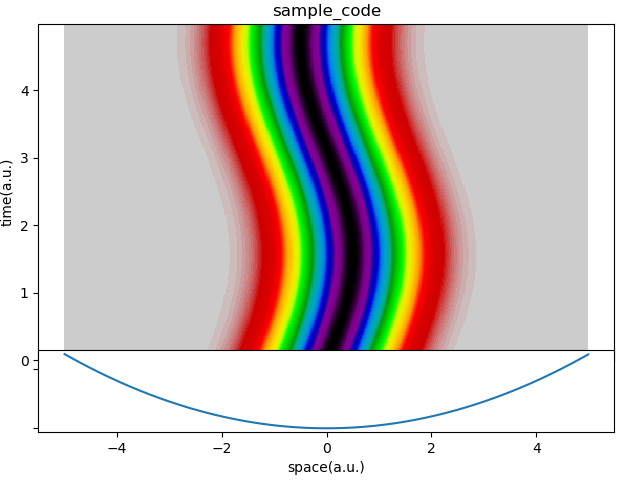
\includegraphics[width=8cm]{sample_code.png}
        \caption{サンプルコード実行結果}
    \end{figure}
    \end{subsection}
\end{section}

\newpage

\begin{section}{QSBのクラス構成\label{AppQ}}
    QuantumSketchBookのオブジェクト(データの構造体)はクラス(メソッドやプロパティのかたまり)としてまとめられている。以下に主要なクラスを示す。
    \begin{itemize}
        \item Mesh:離散化のデータを保持する
        \item Context:Meshを配布する
        \item Field:空間に依存する物理量を表す
        \item Potential:ポテンシャルを表す
        \item State:初期状態を表す
        \item Hamiltonian:ハミルトニアンを表す
        \item Schrodinger:初期値問題を計算する
    \end{itemize}
    \par また, QSB独自概念としてplottableという概念がある。これはQSB付属のplot()関数によって適切なグラフが出力される性質を持つことを指す。
    \par pythonにはPEP8\cite{pep8}によって成文化されたコーディングの指針が存在する。QSBではそれに準じてクラスの頭文字は大文字, 関数, メソッド, プロパティの頭文字は小文字としている。
    \par また, PEP484\cite{pep484}によってタイプヒントというマナーが設定されている(あくまでマナーであるため, 実行時には何の影響も及ぼさない)。これによって, 引数名の後にコロン(:)をつけると, それ以降はデータ型(文字列str, 整数int, 実数numbers.Realなどデータの種類を表すもの)として認識される。QSBでもこのマナーに則り, 引数と返り値の型を明記している。これによって気の利いたテキストエディタを使えば, コンパイル型の言語(cやjavaに代表されるプログラムを実行する前に全てのコードを機械語へ翻訳する形式の言語)のように実行前にエラーを発見することができる。
    \par このセクションにおける次章以降の命名規則を, pythonドキュメントの形式にならって"オブジェクト名(引数名:引数の型, ...)"と定める。デフォルト値(引数が入力されなかった場合に代わりに使用される値)が設定されている引数は"引数名=デフォルト値"と表記する。
    \par 例えばMesh(x\_min: Real, x\_max: Real, dx: Real, t\_min: Real, t\_max, dt: Real)という章は, Meshという名前で引数としてx\_minなどのReal型の6つの引数があるオブジェクトの説明をする章であることを示している。またMeshの頭文字が大文字であることから, このオブジェクトがクラスだということも示している。

    \begin{section}{plot(arg: Plottable, show=True, save=False, title="no\_title")}
        \par plottableなオブジェクト受け取り, 適切な形にプロットされたmatplotlib.Figureを返す。返り値を束縛すれば, 通常のFigureと同様の処理をすることができる。プロットした後のグラフの体裁を変更するための最も一般的な方法という理由で, この返り値の形式が採用されている。
        \par プロットする画像を見る必要がない場合や, 画面にグラフを表示する前にグラフの体裁を変更したい場合には引数showを利用すればよい。引数showがFalseの場合, この関数はmatplotlib.Figureオブジェクトを構成するだけで, 画面にグラフを表示する副作用は発生しない。
        \par また, saveがTrueの場合, プロットされたグラフがtitleと同名のpngファイルとして保存される。titleはファイル名だけでなく, グラフの上部に表示されるグラフタイトルとしても使われる。
        \par matplotlibの仕様によって, 一度作成したFigureは, clear()メソッドを呼び出してメモリを解法しない限り生き残り続ける。一度に大量のグラフを生成する場合は少し注意が必要である。一定以上のFigureが開放されることなく生成されるとmatplotlibはRuntimeWarningを送出する。
        \par plot()関数は内部的にargの\_\_plot\_\_()メソッドを呼び出している。これはpython組み込みのlen(), next(), iter()などと同様の形式である。よって, plottableなクラスを自作したい場合に何か特定のクラスを継承する必要はない。イテレータ(要素を次々と生成できるデータ構造)を自作する場合と同様に, \_\_plot\_\_()メソッドを定義するだけでそのクラスはplottableの性質を持つ。
        \par ただし, plottableなクラスを自作する場合は, \_\_plot\_\_()メソッドは必ずFigureを返さなければならない。これは, 使用者の見えないところでFigureをみだりに生成しないために必要な規則である。一見, いちいちFigureをclearすることは手間であり, \_\_plot\_\_関数内でclearを呼び出す処理をした方が効率的に見える。しかし, そのような仕様では仕様者がグラフの体裁を変更する方法が失われる。また, 見えないところでFigureが生成され, 使用者にとって意図しない効果が起こるよりはclearを明示的に呼び出す方がましなことが多い。これはzen of pythonで知られるPEP20\cite{pep20}の"Explicit is better than implicit."を意識した設計になっている。
    \end{section}

    \newpage

    \begin{subsection}{Mesh(x\_min: Real, x\_max: Real, dx: Real, t\_min: Real, t\_max, dt: Real)}
        \par 時空間の離散化に関するデータを保持する。
        \par Meshの構成過程で物理的に不合理な引数が設定された場合, MeshErrorが送出される。
        \par 様々なオブジェクトが離散化の際にこのクラスを利用するため, 自動でMeshにアクセスできるよう, Contextクラスが提供されている。不慣れな利用者はこちらを使用するべきで, 直接のインスタンス化(具体的なデータを入力してテータ構造を生成すること)は推奨されない。異なったMeshに依存した計算が行われそうになった場合, MeshErrorが送出される。それを避けるためにも後述のContextを通しての使用を推奨する。
        \par Meshはimmutable(一度生成されると変更不可能)という性質を持っている。よって, Meshを変更したい場合は1から新しいMeshを生成しなければならない。しかし, この影響でpythonによって実行時に効率化されたメモリ配置がなされる。この性質によって, 巨大なメッシュを貧弱な計算機でも動かすことができる。また, 辞書のキーや集合の要素としても使用することができる。 
        \begin{table}[h]
            \begin{tabular}{ll}
                プロパティ & 説明\\ \hline
                x\_min & 空間メッシュの最大値\\
                x\_max & 空間メッシュの最小値\\
                dx & 空間メッシュの刻み\\
                x\_vector & 空間メッシュの全要素\\
                x\_num & 空間メッシュの全要素数\\
                t\_min & 時間メッシュの最大値\\
                t\_max & 時間メッシュの最小値\\
                dt & 時間メッシュの刻み\\
                t\_vector & 時間メッシュの全要素\\
                t\_num & 時間メッシュの全要素数\\
            \end{tabular}
        \end{table}
    \end{subsection}

    \begin{subsection}{Context(x\_min: Real, x\_max: Real, dx: Real, t\_min: Real, t\_max, dt: Real)}
        \par Meshの配布を行う。QSBのほとんどのクラスはこのContextが自動生成したMeshを自動で受け取ることができるように作成されているため, 利用者はこのContextをインスタンス化するだけで, 離散化に関する処理を考える必要がなくなる。
        \par 複数のContextが存在する場合, 最後にインスタンス化されたContextの情報が優先されるが, 既に生成されてしまったオブジェクトの情報は更新されないため, Meshを複数使う必要がある場合は異なるMeshに依存したオブジェクトが混在することになる。そこで, Contextの有効範囲を明示化できるようwith構文によるコンテキストマネージャとしての使用法がサポートされている。
        \par with構文は初期化処理と終了処理を隠蔽することができる構文で, Contextの場合はwith構文を抜けたときに自動で最新のContextの情報を消去する終了処理を行っている。そのため, with構文の内側で定義されたオブジェクトは, 必ず互いに同じMeshに依存していることが保証される。
        \par Context.\_\_enter\_\_()メソッド(コンテキストマネージャとして使用された際にpython内部で呼ばれるメソッド)はMeshを返す。as節で束縛することで, Meshを利用することができる。
        \lstinputlisting[caption=Contextの使用例]{context_sample.py}
    \end{subsection}

    \begin{subsection}{Field(arg: Union[Iterable, Callable])}
        \par 空間に依存する物理量を表す。引数にはiterable(イテレータを生成するデータ構造。または, その性質のこと。例:list, set, generator)と一引数の関数のどちらも受け取ることができる。ただし, iterableの要素数と空間メッシュの数が一致しない場合ValueErrorを送出する。
        \par Field内部で各位置での値の情報をMeshと結びつけて保持する。Meshが引数として与えられない場合, Contextから自動的に情報を受け取る。Contextが存在しない場合はMeshContextErrorが送出される。
        \par 抽象クラス(具体的なクラスの基本的な性質だけをまとめたもの)として設計さているため, このクラスを直接インスタンス化することは推奨されない。\_\_plot\_\_()メソッドが定義されているが, valuesという追加の引数から値の解釈を与えなければValueErrorを送出する。
         \begin{table}[h]
            \begin{tabular}{ll}
                プロパティ & 説明\\ \hline
                vector & 各空間メッシュにおける値\\
                mesh & 依存しているMesh
            \end{tabular}
        \end{table}
        \lstinputlisting[caption=Fieldのサンプルコード]{field_sample.py}
    \end{subsection}

    \begin{subsection}{Potential(arg: Union[iterable, function])}
        \par ポテンシャルの情報を保持する。Fieldのサブクラス(親となるクラスのメソッドやプロパティを受け継いだクラス。あるクラスA, Bが"A is a B. "という関係のとき, Aがサブクラス, Bが親クラスに当たる)のため, Fieldと同様に配列と関数のどちらも受け取ることができる。また, 具体的なPotentialを構成するための関数(box(), step(), kp()など)がいくつか用意されている。これらの基本的なポテンシャルを組み合わせても, 任意のポテンシャルを表すPotentialクラスのインスタンスを作ることができる。
        \par このクラスではスカラー倍とポテンシャル同士の加減がサポートされている。スカラー倍ではすべての位置におけるポテンシャルがスカラー倍される。ポテンシャル同士の加減では, 各位置におけるポテンシャルの値の和差がとられる。
        \par plottableの性質を持つため, plot(some\_potential)とすれば, 簡単にグラフを作成できる。
        \par matrix()メソッドは疎行列の形で行列要素を返すため, 巨大なMeshであっても$O(n)$のオーダーでメモリを使うことができる。素直な実装では$O(n^2)$の保存領域を使うため, すぐにメモリを使いきってしまう。
        \begin{table}[h]
            \begin{tabular}{ll}
                プロパティ & 説明\\ \hline
                matrix() & ポテンシャルの行列要素を返す\\
            \end{tabular}
        \end{table}
        \lstinputlisting[caption=Potentialの使用例]{potential_sample.py}
        使用例を実行すると以下のグラフが出力される。
        \begin{figure}[h]
            \begin{minipage}{0.5\hsize}
                \centering
                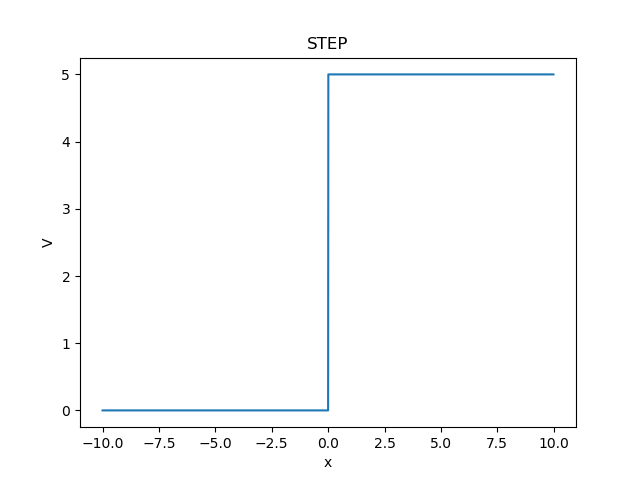
\includegraphics[width=0.9\hsize]{STEP.png}
                \caption{ステップポテンシャル}
            \end{minipage}
            \begin{minipage}{0.5\hsize}
                \centering
                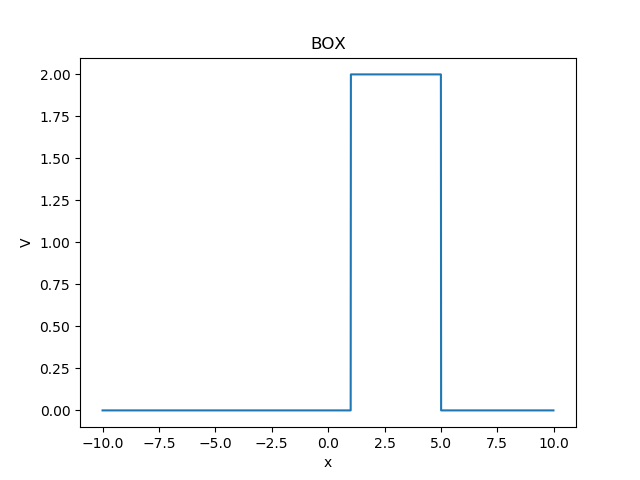
\includegraphics[width=0.9\hsize]{BOX.png}
                \caption{箱型ポテンシャル}
            \end{minipage}\\
            \begin{minipage}{0.5\hsize}
                \centering
                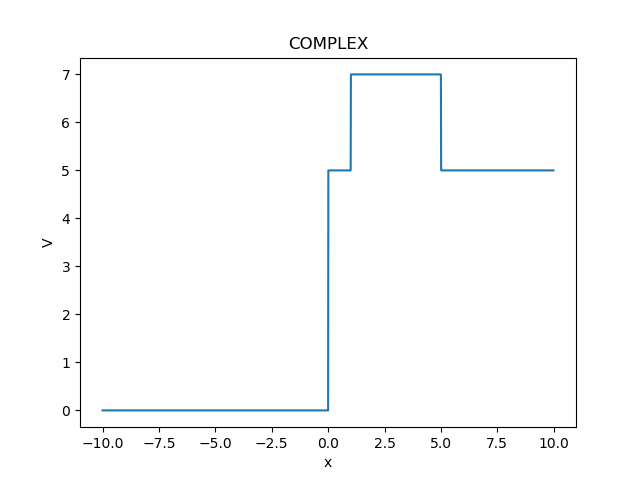
\includegraphics[width=0.9\hsize]{COMPLEX.png}
                \caption{ポテンシャルの足し合わせ}
            \end{minipage}
            \begin{minipage}{0.5\hsize}
                \centering
                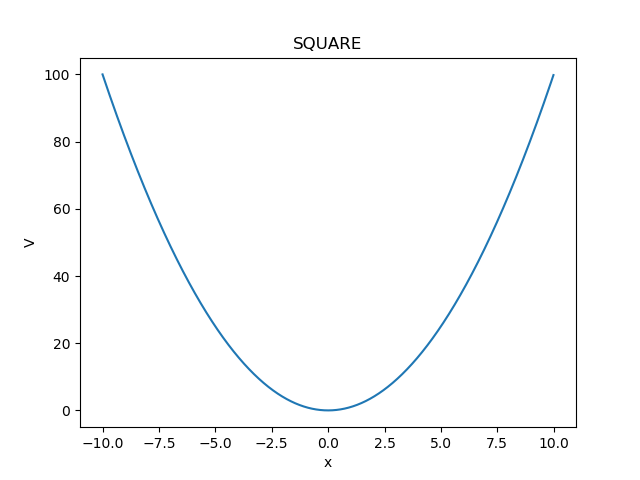
\includegraphics[width=0.9\hsize]{SQUARE.png}
                \caption{二次関数}
            \end{minipage}\\
            \begin{minipage}{0.5\hsize}
                \centering
                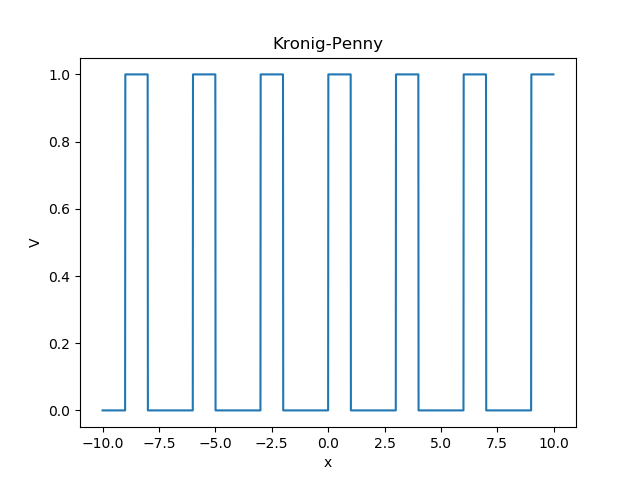
\includegraphics[width=0.9\hsize]{Kronig-Penny.png}
                \caption{Kronig-Pennyポテンシャル}
            \end{minipage}
            \begin{minipage}{0.5\hsize}
                \centering
                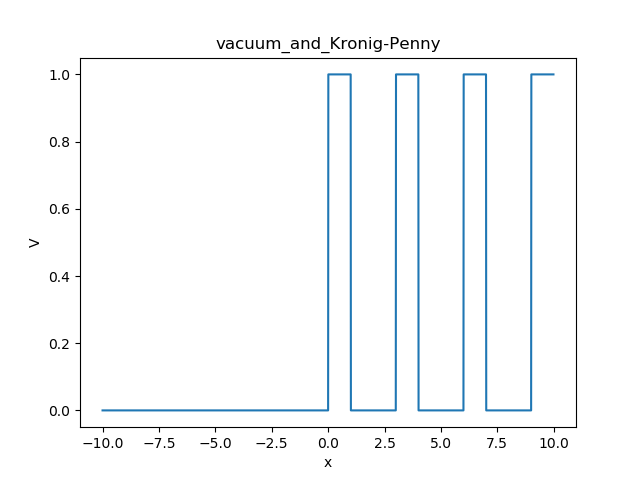
\includegraphics[width=0.9\hsize]{vacuum_and_Kronig-Penny.png}
                \caption{真空とKronig-Pennyポテンシャル}
            \end{minipage}
        \end{figure}
    \end{subsection}

    \begin{subsection}{State(arg: Union[iterable, function])}
        \par 初期状態に関する情報を保持する。Fieldのサブクラスのため, 配列と関数を受け取ることができる。
        \par random\_values(n)メソッドを使うとStateの確率密度分布に従うn個の乱数を生成することができる。これはNelsonの確率過程を生成する際の初期値を得るために使われる。乱数生成にはvon Neumannの棄却法を用いている。
        \par plottableであるため, plot(some\_state)とすれば, グラフを作成できる。
        \par Gauss型波束のStateを構成するための関数gaussian\_state()が用意されている。
        \lstinputlisting[caption=Stateの使用例]{state_sample.py}
         使用例を実行すると以下のグラフが得られる。プロットされているものが確率密度分布だということには注意が必要だと考えられる。波動関数の標準偏差が3のとき, 絶対値2乗をとった確率密度分布の標準偏差は1.5になる。
         \begin{figure}[h]
            \centering
            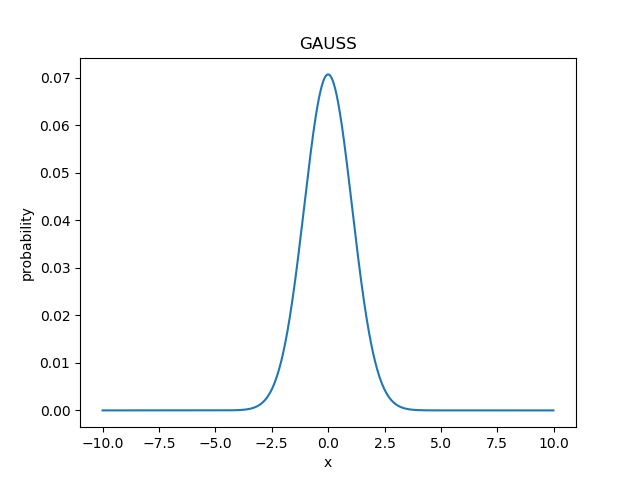
\includegraphics[width=8cm]{GAUSS.png}
            \caption{Gauss型波束}
        \end{figure}
    \end{subsection}

    \begin{subsection}{Hamiltonian(potential: Potential, boundary="free")}
        \par Potentialを受け取って, ハミルトニアン演算子を保持する。
        \par 境界条件の指定はこのクラスの引数によって行われる。指定可能な境界条件は挙動が安定している自由端境界条件"free", 固定端境界条件"fix", 周期境界条件"period"の3種類と, 試験的に導入されている吸収境界条件"absorb"を合わせた4種類である。それ以外を指定した場合一部の例外を除いて, ValueErrorが送出される。デフォルト値は"free"に設定されている。
        \par 境界条件は, 本来の意味合い的には時空を管理するMeshに保持させるべきものである。しかし, 同様のMeshを使った異なる境界条件での計算を行う場面を考慮して, 変更不能で多くのデータの基礎となっているMeshではなく, 比較的変更しやすいHamiltonianに保持させる形になっている。また, 物理的にも, Schrödinger方程式の境界条件はハミルトニアンの行列要素に反映されるため, 大きく的を外した仕様ではない。
        \par 行列要素は疎行列によって保持されている。これによって, Potentialの場合と同様に, 素直な実装では$O(n^2)$のメモリを使うところを$O(n)$に抑えている。また, 行列積の計算に疎行列用の効率化されたメソッドを使うことができるため, 計算時間も短縮される。よって, このクラスではメモリ, 時間ともに効率化されているといえる。
        \par QSBを使用する分には気にする必要性はないが, scipyに付属されている微分方程式ソルバーは一変数関数の一階微分方程式しか解くことができない。一方, 波動関数は位置と時間とで二つの変数を持つため, そのままではscipyを使ってSchrödinger方程式の求積計算をすることができない。そこで, QSBでは各メッシュ点における波動関数をすべて独立な変数とみなし, 全ての変数について連立した微分方程式を作ることでこの問題を解決している。
        \par Hamiltonianの実態は連立微分方程式の係数を保持する役割を担うものである。これは物理的には空間表示したハミルトニアンの行列要素を保持することに対応している。冒頭で述べたハミルトニアン演算子を保持するとは, 厳密にはハミルトニアンの行列要素を保持することを指している。
        \par 使用例は次章のSchroedingerの使用例で一緒に例示する。
        \begin{table}[h]
            \begin{tabular}{ll}
                プロパティ & 説明\\ \hline
                matrix & ハミルトニアンの行列要素を返す\\
            \end{tabular}
        \end{table}
    \end{subsection}

    \begin{subsection}{Schroedinger(hamiltonan: Hamiltonian, state: State)}
        \par 初期値問題の求解を行う。HamiltonianとStateを受け取ってSchrödinger方程式の数値解を保持する。
        \par 積分器はscipy.integrate.odeを通して, Fortranサブモジュールの一つであるzvodeを指定している。注意として, zvodeはscipyの仕様で2つ以上のインスタンスを同時に作ることはできないとされている。よって, QSBでも, 必ず一つの方程式を解き終えてから別の方程式を解かせるように使用しなければならない。zvodeはnon-stiffな問題に対して予測子修正子Adams法を使い, stiffな問題に対して後退差分法を使う。一般に予測子修正子Adams法のほうが精度が高く, 高速に計算できる。
        \par 計算量を節約しようとするときに計算範囲を狭くすることがあるが, 初期状態で波束の一部が計算範囲からはみ出してしまうと, 問題がstiffになり, zvodeが後退差分法を適用してしまうため, 逆に計算量が増加してしまう場合がある。
        \par 計算範囲を広げすぎてしまうと余分な計算が増えるため, なるべく小さなメッシュを使用すべきなことに間違いはない。しかし, 波動関数がほとんどの場所で0になるような場合, 乗算のコストはあまり高くない。広範囲に広がらない波束のような状態の時間発展を計算する場合は, メッシュ範囲の大きさに敏感になる必要はあまりない。
        \par 数値解は初めてSchroedinger.solution()メソッドが呼び出されたときに計算され, キャッシュされる。よって, 二回目以降の呼び出しは高速になる。 また, Schrodeingerはiterableであり, 各ステップでの解を順々に返すことができる。この機能はMeshが巨大すぎて全ての時間に渡る解を一度にメモリに乗せることができない場合の対抗策として設計されている。
        \par Schroedingerがiterableとして呼び出された場合は, 過去のステップで保持されたメモリが次のステップを呼び出すとすぐに開放される。そのため, 1ステップ分のデータがメモリの上に乗ればどれだけ長時間に渡る計算であってもメモリエラーを起こさず実行することができる。
        \par デフォルトのラプラシアンは\eref{QSBeq}の形式を採用した。
        \begin{align}
            \Delta := \frac{1}{360\varDelta x^2} \left(4\phi_{i-3} - 54\phi_{i-2} + 540\phi_{i-1} - 980\phi_{i} + 540\phi_{i+1} - 54\phi{i+2} + 4\phi_{i+3}\right)\label{QSBeq}
        \end{align}
        ただし$\phi_i$はメッシュ番号$i$における波動関数で, $\varDelta x$は空間メッシュの間隔。境界値では境界条件に従って係数を変化させている。
        \par \eref{QSBeq}をtight-bindingモデルで解釈すると, 滑らかな空間における3格子点先の飛び移りまでを考慮に入れることに対応している。
        \par この形式は$\phi_i$の左右3点と$\phi_i$自身を含む7点をRagrange補間し, 2回微分することで得られる。7点を与えたRagrange補間は$\phi_i$周辺を6次の精度で近似できるため, それを2階微分した\eref{QSBeq}は$O(\varDelta x^4)$の精度がある。ただし, 等間隔メッシュで高次のRagrange補間を行うと, 近似した関数が激しく波打つRunge現象が起こるため, 安心して精度が高いと言えるのは$\phi_i$のごく周辺だけである。
        \par QSBでは境界条件に"poor"と入力すると1次の精度がある公式と入れ替えられるように設計されている。
        \par Hamiltonianはplottableであり, plotすると$x-t$パターンとポテンシャルのグラフを生成する。プロットエリア上部に$x-t$パターンが描写され, プロットエリア下部にポテンシャルのグラフが描画される。
        \begin{table}[h]
            \begin{tabular}{ll}
                プロパティ & 説明\\ \hline
                mesh & 依存しているMesh\\
                potential & 依存しているPotential\\
                x0state & 依存しているState\\
                ode & 微分方程式のソルバー\\
                equation(t, phi0) & odeによって解かれる方程式をメソッド化したもの\\
                solution() & Schrödinger方程式の解を返す。2回め以降はキャッシュを用いるため高速\\
                nelson() & Nelsonの確率過程の標本を生成するためのNelsonクラスオブジェクトを生成する\\
            \end{tabular}
        \end{table}
        \lstinputlisting[caption=HamiltonianとSchroedingerの使用例]{schroedinger_sample.py}
        使用例を実行すると以下のグラフが出力され, 実行場所にpng形式のファイルが保存される。
        \begin{figure}[h]
            \begin{minipage}{0.5\hsize}
                \centering
                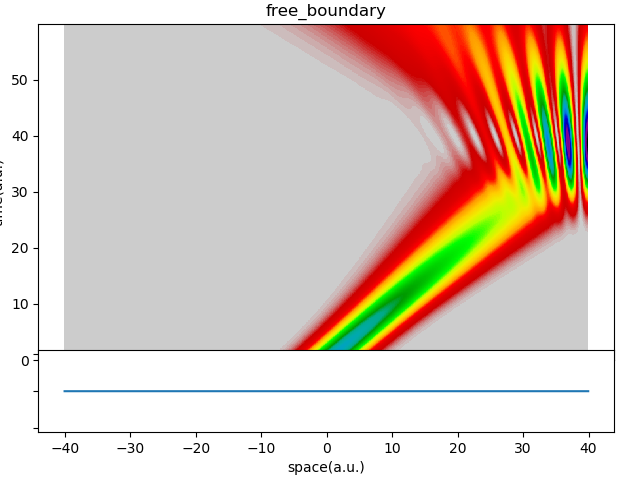
\includegraphics[width=0.9\hsize]{free_boundary.png}
                \caption{自由端境界条件}
                \label{free}
            \end{minipage}
            \begin{minipage}{0.5\hsize}
                \centering
                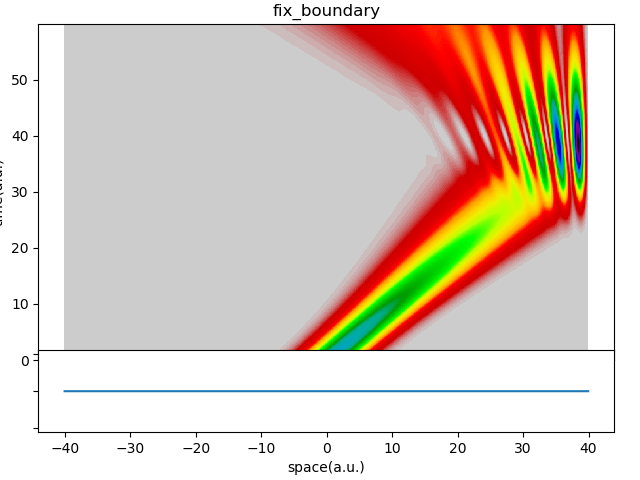
\includegraphics[width=0.9\hsize]{fix_boundary.png}
                \caption{固定端境界条件}
                \label{fix}
            \end{minipage}\\\\\\
            \begin{minipage}{0.5\hsize}
                \centering
                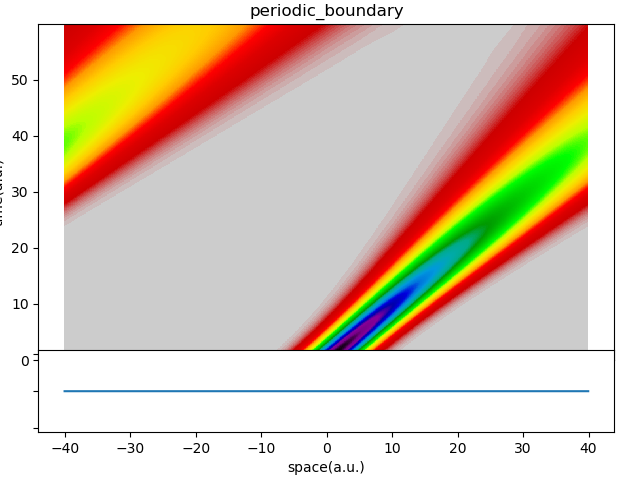
\includegraphics[width=0.9\hsize]{periodic_boundary.png}
                \caption{周期境界条件}
                \label{period}
            \end{minipage}
            \begin{minipage}{0.5\hsize}
                \centering
                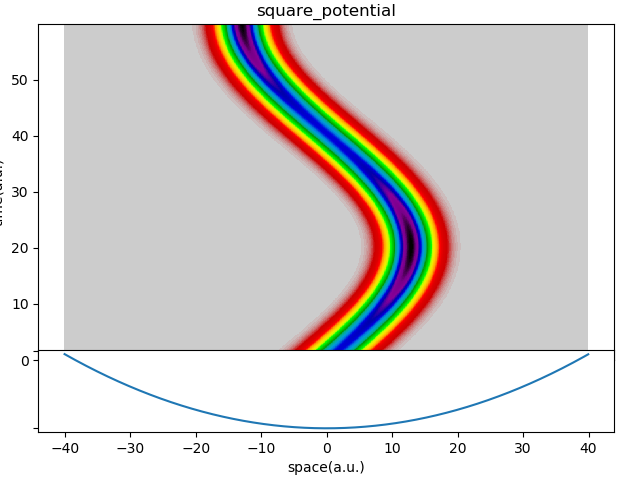
\includegraphics[width=0.9\hsize]{square_potential.png}
                \caption{2次関数}
            \end{minipage}\\
        \end{figure}
        \par \fref{period}の境界条件による影響はその他の境界条件と区別しやすいが, \fref{free}と\fref{fix}も境界での反射の仕方が微妙に異なっている。具体的には, \fref{free}は反射の際に必ず境界が着色される(確率が高いことを表す)が, \fref{fix}は絶対に境界が着色されない。
        \par 2次関数ポテンシャルの例では波束がほとんど緩和しない。これはSchrödinger方程式の定常解から考えても自然なことだと考えられる。また, 波束が左右に行ったり来たりする様子は, 古典的な質点の振る舞いとも一致する。これらの定性的特徴はQSBによってSchrödinger方程式の求解ができていることを示す一つの証拠と言える。
    \end{subsection}

\end{section}

\begin{section}{QSBの妥当性検証}
    QSBの妥当性検証のため, Zhangの論文にあるHeyperdiffusionの場合についてQSBを用いた計算を行った。この章ではHeyperdiffusionについての簡単な解説とZhangの行った計算の設定を紹介し, 最後にQSBによる計算結果を示す。

    \begin{subsection}{Heyperdiffusion}
        \par Heyperdiffusionは拡散現象の形態の一つで, 分散$\sigma^2$が時間$t$に関して\eref{Heyperdiffusion}の形で拡散することをいう。
        \begin{align}
            \sigma^2 &\propto t^\alpha \label{Heyperdiffusion}\\
            2 &< \alpha
        \end{align}
        ブラウン運動的な拡散は$\alpha=2$で拡散するため, Heyperdiffusionはブラウン運動を越える拡散のことだといえる。
        \par Schrödinger方程式に従う真空中のGauss型波束も同様に$t^2$に比例した速さで分散が増加する。よって, ポテンシャル中の量子波束がHeyperdiffusionを起こすということは真空中よりも高い次数に比例して拡散していくことと等しい。もちろん, 比例定数が異なるため, 単純に次数が大きい, 即ち速く拡散しているとはいえないが, 素朴な直感に反することは事実である。
        \par この現象の理論的な説明の一つとしてHufnagel\cite{Huf}のpoint-sourceモデルによる説明を紹介する。このモデルでは, x=0に集中した確率の源が, 指数関数的に減衰する様子を\eref{source}の形で仮定する。
        \begin{align}
            P(t) = \mathrm{e}^{-\Gamma t}\label{source}
        \end{align}
        \par ここで$P(t)$は, x=0に粒子が存在する確率を表す。$\Gamma$は拡散のスケールを表す正の定数。x=0の位置から失われた粒子が, 等速で周囲に拡散していくと仮定すると, \eref{variant}のように分散$M_{PS}(t)$を計算することができる。
        \begin{align}
            M_{PS}(t)&=\int_{0}^{\infty}\:dx\:x^2\int_{0}^{t}\:dt'(-\dot{P}(t'))\delta(x-v(t-t'))\label{variant}\\
            &=v^2\Gamma\int_{0}^{t}\:dt'\mathrm{e}^{-\Gamma t}(t-t')^2\nonumber\\
            &=v^2\left(t^2-\frac{2}{\Gamma}t+\frac{2}{\Gamma^2}-\frac{2}{\Gamma^2}\mathrm{e}^{-\Gamma t} \right)\label{MPS}
        \end{align}
        \par \eref{MPS}の1項目は通常のブラウン運動的拡散を表すが, 2項目以降の項はそれと異なる影響を表している。$t<<\Gamma$というゆっくりとした拡散の状況では2項目以降は打ち消し合うため, ブラウン運動と一致する。一方, $t\sim\Gamma$の状況ではこれらの項が無視できない影響を与えるため, 異常な拡散の挙動を示す。Hufnagelはこの拡散をHeyperballisticな拡散と呼んだ。
    \end{subsection}

    \begin{subsection}{Zhangの研究結果の再現}
        \par Zhangの研究では主格子の内部に副格子が存在している構造のポテンシャルを使用している。主格子がHufnagelの言うところのpoint-sourceに対応する。
        \par 主格子は箱状で, 格子番号を$i$としたとき$m\in [-L, L]$となるように設定されている。Zhanの計算では主に$L=50$としているため, 今回の再現もそれにならった。
        \par 主格子内のポテンシャル構造は副格子の構造によって決定される。Zhangが行った周期的なポテンシャルにおける計算の中では$V=V_0 (-1)^i$を使用していた。ここで$V_0$はポテンシャルの高さを決定する因子で, 0.0, 1.0, 1.5, 1.9, 2.0がZhangの論文では発表されている。
        \par 初期条件$\phi_0$はKroneckerのデルタ型の波束$\delta_{0, i}$を使用していた。
        \par ハミルトニアン内に含まれるラプラシアンについては\eref{1ji}を使用している。
        \begin{align}
            \Delta \phi_i := \frac{\phi_{i-1} - 2\phi_{i} + \phi_{i+1}}{\varDelta x^2}\label{1ji}
        \end{align}
        \par この式は$O(\varDelta x)$の精度がある\cite{Carnahan}。
        \par また, tight-bindingモデルで解釈すると, 1次の飛び移りまでを考慮することに対応する。格子間の飛び移りがQSBで再現する際は, Hamiltonianに一次精度のラプラシアンを使うように指定した。
        \par QSBで上記のラプラシアンを用いた$i\in [0, 10^4]$について自由端境界条件をつけて$t<10^4$ステップに渡り時間発展を計算したところ, 分散は\fref{bunsan}のように時間発展した。個別のケースの計算には各2時間程度を要した。
         \begin{figure}[h]
            \centering
            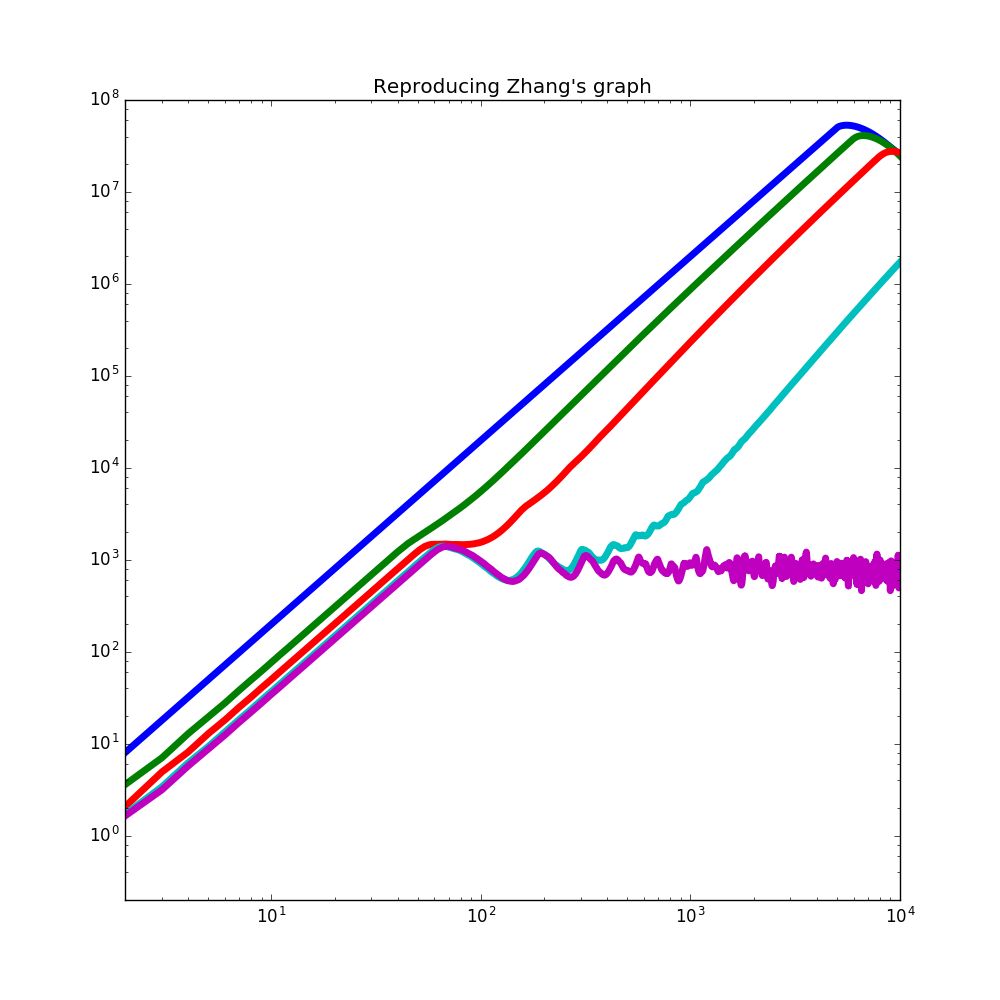
\includegraphics[width=8cm]{zhang.png}
            \caption{波束の分散の時間推移}
             \label{bunsan}
        \end{figure}
        \par 線の色はそれぞれ上から$V_0$=0.0, 1.0, 1,5, 1,9, 2.0に対応している。
        \par 縦軸は分散を表し, 横軸は時刻を表している。両対数軸をとっているため, グラフの傾きが多項式近似した際の次数に対応する。縦軸と横軸の比は2:1であるため, 通常のブラウン運動的拡散でのグラフは傾き45度の直線となる。Heyperdiffusionが起こるとグラフの傾きが45度を超えるものが現れる。
        \par \fref{bunsan}の特徴として, 傾きが45度を超え, 分散が$t^\alpha(\alpha>2)$に比例して増加する現象が見られた。これはHeyperdiffusionの特徴と一致している。長時間での分散の値が増加していないのは境界に達した波動関数が反射した影響だと考えられる。
        \par 同じ縮尺のグラフをコンピュータ上で重ねたところ, 境界条件の影響を除けば, Zhangの作成したグラフの線の上にQSBのグラフの線が重なることを定性的に確認できた。
        \par また, 最小二乗法フフィッティングにより, Zhangの報告している$\alpha$と一致する値が定量的に得られた。各パターンでの$\alpha$を以下に示す。
        \begin{table}[h]
            \begin{tabular}{lcc}
                V&QSB & Zang\\ \hline
                0.0&2.00&2\\
                1.0&2.23&2.2\\
                1.5&2.39&2.4\\
                1.9&2.58&2.6
            \end{tabular}
        \end{table}
        \par これによって, Zhangの計算とQSBの計算が一致したということが確認できた。以降の計算も妥当であるという前提で解釈を行う。
    \end{subsection}
\end{section}

\newpage

\begin{section}{条件設定}
    \par 数値計算におけるパラメータを以下のように設定してQSBによる計算を行った。
    \par 空間の離散化のパラメータは$x\in [-60, 60]$で, $\varDelta x=0.05$のメッシュに自由端境界条件を採用した。時間の離散化パラメータは$t\in [0, 30]$で$\varDelta t=0.05$とした。
    \par 初期条件はGauss型波束$\mathrm{std}(x_0, \sigma, x)\mathrm{exp}[ikx]$を使用した。パラメータは平均値$x_0=-15.00$標準偏差$\sigma=6.00$平均波数$k=2.00$に設定した。標準偏差は波動関数のもので, 確率密度の標準偏差は3.00となる。
    \par 波束の状態を固定する理由は, 波束の拡散現象がスケール不変なことにある。波束の平均波数を変えても, ポテンシャルと時間, 空間のスケールを変換することで同じ状況に対応させられる。標準偏差を拡大することは, 空間のスケールを縮小し, 時間のスケールを拡大することに対応する。よって, 波束を固定し, ポテンシャルを変えるだけでポテンシャルと波束の対応関係を見る分には十分である。
    \par ポテンシャルを固定して波束を変化させる方法を取らない理由は, 波数を大きくすると計算領域の境界にたどり着いてしまう可能性が高くなったり, 時間スケールを拡大するためにメッシュを変更することには余分なコストがかったりとQSBで数値計算する上でのデメリットが多いからである。
    \par 周期ポテンシャルは以下のように設定した。
    \begin{align}
     V(x)=\begin{cases}0&(x<0)\\V_{KP}(x)&(x>0)\end{cases}\nonumber\\
    \end{align}
    \par 実際の数値計算では, QSBのvacuum\_kp()関数を用いた。
    \par $V_{KP}(x)$には3つのパラメータ$a, b, V_0$があるため, 本研究で使用するポテンシャルもこれらの3つのパラメータによって完全に決定される。本研究の計算ケースはポテンシャルにのみ依存するため, これらの3つのパラメータの組み合わせによって各計算パターンは特徴づけられる。
    \begin{subsection}{物理的状況の考察}
        \par 上記の設定は$x<0$の真空領域から, $x>0$の周期ポテンシャル領域に平均波数2.00で入射する波束を想定している。
        \par 実際の結晶表面はダングリングボンドや格子欠損のような表面特有の現象が起こるが, このモデルではその影響は含まれていない。また, 実際の結晶中分子が作るポテンシャルはKronig-Pennyポテンシャルのような切り立った傾きで立ち上がっていない。飽くまでKronig-Penny型の周期ポテンシャルに入射する電子波束を想定している。
        \par 平均波数2.00は真空中の平面波において2.00単位エネルギーを持つ状態で, 丸め誤差の範囲内でde Broglie波長$\pi$に対応している。
        \par $V_0=0$の状況では$t=30$の時点で波束中心は$x=45.00$にあり, 約片側$2\sigma$が計算範囲内に入る。
        \par $v_0>0$の状況では真空の状況よりも波束の伝搬が遅くなるため, 一般に$x=60$の境界で反射する粒子は2.5\%を上回らない。
        \par また, 境界で反射した粒子がもう一度$x<0$の領域に侵入する確率は$10^{-10}$を下回ると推定される。
    \end{subsection}
\end{section}

\newpage

\begin{section}{結果}
    \begin{subsection}{x-tパターン\label{x-tpatturn}}
        \par QSBによって5000ケース以上のケースについて計算し, 得られた波束の時間発展を$x-t$パターンの形式で図示した。
        \par $x-t$パターンは各時刻における各位置の存在確率を色で表したもので, 古典力学で用いられる$x-t$グラフの拡張として捉えることができる。軌跡の傾きは古典的な速度に対応するが, 量子力学では量子が確率的な広がりを持つため, 軌跡を大まかにしか見取ることはできない。
        \begin{figure}[h]
            \centering
            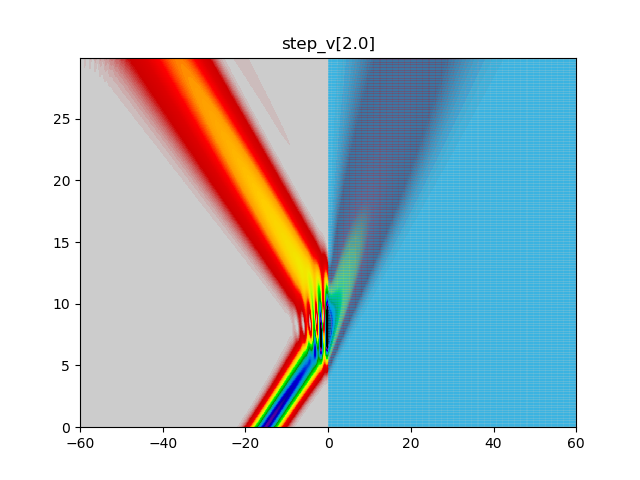
\includegraphics[width=\hsize]{rei.png}
            \caption{$x-t$パターンの例:ステップポテンシャルに入射する波束をシミュレーションしたもの}
            \label{example}
        \end{figure}
        \par 縦軸は時刻, 横軸は位置を表している。紫の領域の確率密度が最も高く, 青緑黄赤の順に低くなっていく。灰色の領域は確率が0の領域を表している。半透明の水色で塗られた領域は壁を意味するが, 色は全て同じで, ポテンシャルの高さとは対応していない。
        \par \fref{example}では右側のポテンシャル領域に入射した波束が5から10単位時間ごろにポテンシャル表面で反射し, 左側に伝搬していくものと, ポテンシャル領域に侵入していくものとに分かれる様子が確認できる。
        \par ポテンシャルに侵入した進行波の軌跡の傾きが急になっていることから, 伝搬速度が遅くなっている様子も確認できる。
        \par 反射波の方は時間経過と共に黄色の領域が少なくなり赤の領域が増していることから, 波束が緩和している様子を確認することができる。
        \par $x-t$パターンはこのように多くの情報をアニメーションに頼らずに得ることができるため, 量子力学的な現象であっても時間発展の様子を知るための道具として優れている。アニメーションは計算機での生成コストが高く, 大量に作ることが困難である。また, 人間がアニメーションを観る際には再生時間が必要で, 大量のデータを処理することにも向いていない。読解に少しコツが必要だが, 大量のケースについて読解する必要がある場合は$x-t$パターンのほうが適切だと考えられる。
        \par 次章以降ではシミュレーションによって得られた以下の特徴的な$x-t$パターンを例示する。
        \begin{itemize}
            \item 全反射
            \item 高次反射波
            \item 高次進行波
            \item 分裂状態
            \item 屈折状態
            \item トラップ状態
            \item 停滞状態
        \end{itemize}
    \end{subsection}

    \begin{subsection}{全反射}
        \begin{figure}[h]
            \centering
            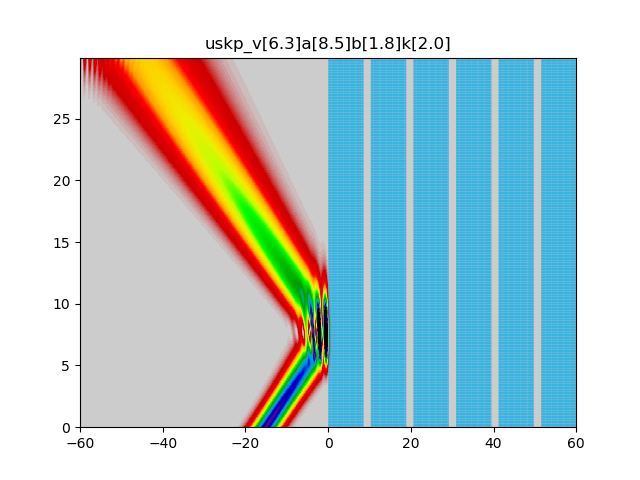
\includegraphics[width=8cm]{zenhansha.png}
            \caption{全反射の例$V_0$=6.3, a=8.5, b=1.8の場合}
        \end{figure}
    \par 壁が厚すぎたり, ポテンシャルが高すぎたりする場合にみられる。ほとんどの波が反射する。ポテンシャルの高さは2よりも大きくなければ現れない。逆にポテンシャルの高さが5を超えると, 全反射以外のパターンが現れることは稀になる。
    \par$x-t$パターン上では, どの個別ケースもほぼ同じような形状をしているため, 複数の例示はしない。
    \par ポテンシャルの高さが2よりも小さい場合は入射エネルギーよりもポテンシャルのほうが低いため, ポテンシャルに侵入する波束が現れ, 全反射パターンは現れなくなる。その代わりに停滞状態が多くを占める。
    \end{subsection}

    \begin{subsection}{停滞状態\label{teitais}}
        \begin{figure}[h]
            \begin{minipage}{0.5\hsize}
                \centering
                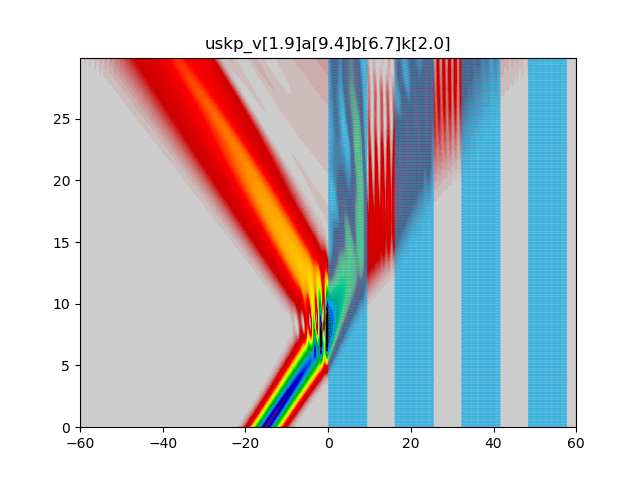
\includegraphics[width=0.9\hsize]{teitai1.png}
                \caption{停滞状態の例:典型的なもの$V_0$=1.9, a=9.4, b=6.7}
                \label{teitai1}
            \end{minipage}
            \begin{minipage}{0.5\hsize}
                \centering
                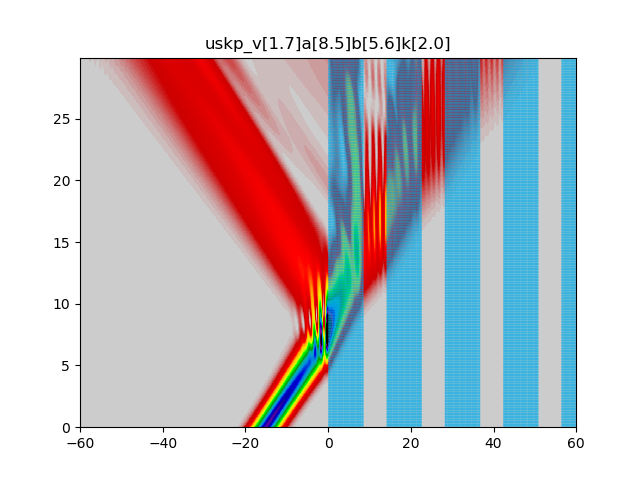
\includegraphics[width=0.9\hsize]{teitai2.png}
                \caption{停滞状態の例:2層目でも黄色い領域が見られる$V_0$=1.7, a=8.5, b=5.6}
                \label{teitai2}
            \end{minipage}\\
            \begin{minipage}{0.5\hsize}
                \centering
                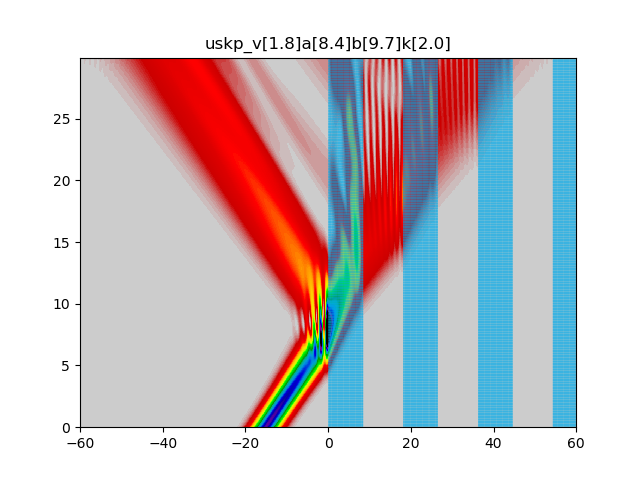
\includegraphics[width=0.9\hsize]{teitai3.png}
                \caption{停滞状態の例:1層目壁内部で2回真空領域に反射している$V_0$=1.8, a=8.4, b=9.7}
                \label{hanshamiyasui}
            \end{minipage}
            \begin{minipage}{0.5\hsize}
                \centering
                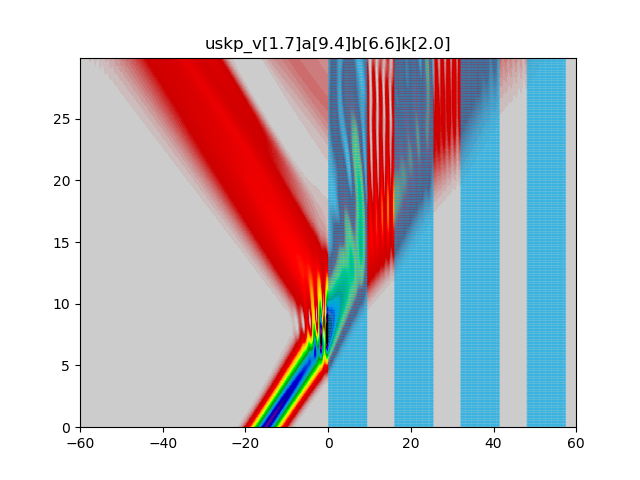
\includegraphics[width=0.9\hsize]{teitai4.png}
                \caption{停滞状態の例:観測した中で停滞時間が最長のもの$V_0$=1.7, a=9.4, b=6.6}
                \label{teitai3}
            \end{minipage}
        \end{figure}
        \par ポテンシャルが2より低く, 壁が5よりも厚い場合に分かりやすいものが現れる。井戸ではなく壁の領域に注目すると, 壁内部にとどまり続ける波が存在している。
        \par ポテンシャルが2よりも低い設定では多かれ少なかれ必ずこの状態の影響が見られる。停滞状態はポテンシャルが2を超えると段々と見られなくなり, 3を超えるとほとんどの影響が見られなくなる。壁が厚ければ厚いほど内部に波が留まりやすい。
        \par 素朴に考えるとポテンシャルが高い領域に存在する確率は低くなりそうだが, シミュレーション結果では井戸よりも壁に多く確率が集まる様子が確認できた。
        \par ポテンシャルが高い領域に確率が集まる現象は, 後述するが, 箱型ポテンシャルにも見られる。
        \par \fref{hanshamiyasui}の時刻20単位時間ごろのポテンシャル境界付近に注目すると分かりやすいが, 壁にとどまる波の一部は真空方向へ反射する。しかし, 波束の軌跡は大きく弧を描くように曲がっており, 時間をかけて反射していく様子が見受けられる。
        \par 壁内部に停滞する波束は, かなり大きい時間スケールで周囲の真空や井戸に拡散していく。この影響で, 真空側の反射波は波束のようなまとまった形は取らず, 散発的に壁から放出されていくものが現れる。
        \par 一枚の壁からどの程度の時間をかけて放出されて行くのかを調べるため, 箱型ポテンシャルに同様の波束を入射したところ, \fref{hako_short}のような$x-t$パターンを得た。
        \begin{figure}[h]
            \centering
            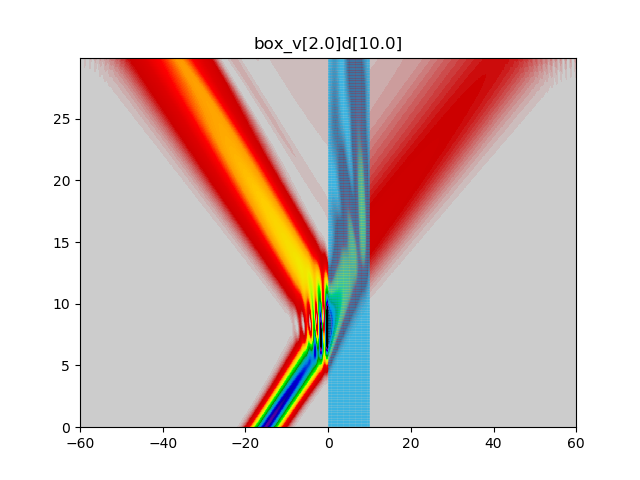
\includegraphics[width=10cm]{hako_short.png}
            \caption{箱型ポテンシャルに入射した波束の時間発展$V$=2.0}
            \label{hako_short}
        \end{figure}
        \par 壁の内部にとどまり続ける波が観察できる。ゆっくりと弧を描くように反射する様子も, 周期的に並んでいる場合と同様の傾向が見受けられた。\fref{hako_short}を更に3倍の時間について時間発展を計算すると\fref{hako_long}が得られた。
        \begin{figure}[h]
            \centering
            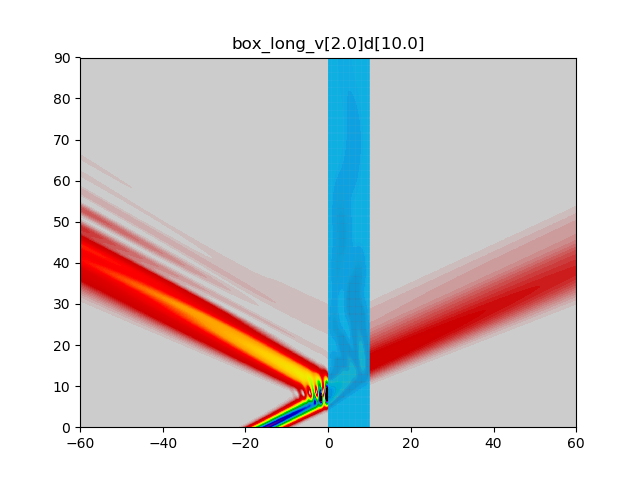
\includegraphics[width=10cm]{hako_long.png}
            \caption{90単位時間まで計算された箱型ポテンシャルにおける時間発展}
            \label{hako_long}
        \end{figure}
        \par 境界の影響を排除するため, 画像には描かれていないが, 空間メッシュを3倍に広げて計算している。
        \par \fref{hako_long}では壁内部に80時間程度まで停滞する様子が見受けられる。着色する閾値以下ではさらに停滞していると考えられる。
        \par このように壁内部に長時間滞在し, ゆっくりと時間をかけて外部に放出する影響で, 次章以降に示すパターンにはポテンシャル境界での反射では説明できないノイズのようなものが混入する。停滞の影響を受ける, 受けないで波束の振る舞いはかなり違ったものになるため, ポテンシャルが2より大きいか小さいかは波束の時間発展を決める上で重要な因子となる。
        \par 壁内部の滞在時間が長くなること理論的な間接証拠として, 箱型ポテンシャル定常状態における壁内部と真空の確率密度の比を\fref{hako_in}に示す。
         \begin{figure}[h]
            \centering
            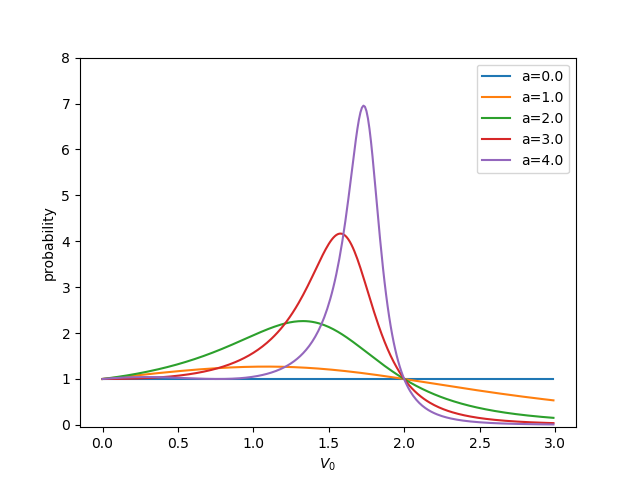
\includegraphics[width=10cm]{hako_in.png}
            \caption{真空領域の滞在確率/壁内部の滞在確率}
             \label{hako_in}
        \end{figure}
        \par 系のエネルギーはシミュレーションにおける平均エネルギーと等しい2に設定してある。
        \par 横軸はポテンシャルの高さ, 縦軸は真空領域の確率密度/ポテンシャル領域の確率密度を表している。縦軸が1を超えた場合, 粒子が見いだされる確率密度はポテンシャル領域のほうが高いことを意味している。aはKronig-Pennyモデルと同様に壁の厚さを表している。
        \par \fref{hako_in}から, $V_0<2$の領域では壁内部のほうが確率密度が高くなっていることがわかる。また, $V_0$が2よりも少しだけ小さいときに現れるピークは壁の厚さを表す$a$が大きくなるほど鋭くなる。
        \par よって, 入射エネルギーよりも少しだけ低いポテンシャルでは, aの値が大きくなるごとに滞在時間が増えていくことがいえる。この傾向はシミュレーションでポテンシャルを2周辺に設定したときに, 壁が厚くなるほど停滞し続けるという停滞状態の傾向と一致している。このことから, Kronig-Pennyポテンシャルにおけるシミュレーションでも同様の傾向があると考えられる。
        \par また, 直感的な説明として壁内部の伝搬速度を使う説明が考えられる。箱型ポテンシャルの場合, 壁内部の位相速度は準波数に比例する。順波数はエネルギーを$\varepsilon$としたとき, 準波数は$\sqrt{2m(\varepsilon - V_0)}$となるため, $\varepsilon \sim V_0$の状況では, ほぼ0になる。伝搬速度もほぼ0になるため, 粒子は長時間壁内部に滞在し続けると説明できる。
        \par ただし, 波束の場合は様々な波数の波が重なり合っているため, 壁内部で完全に停止する粒子は現れない。
    \end{subsection}

    \begin{subsection}{高次反射波}
     \begin{figure}[h]
        \begin{minipage}{0.5\hsize}
            \centering
            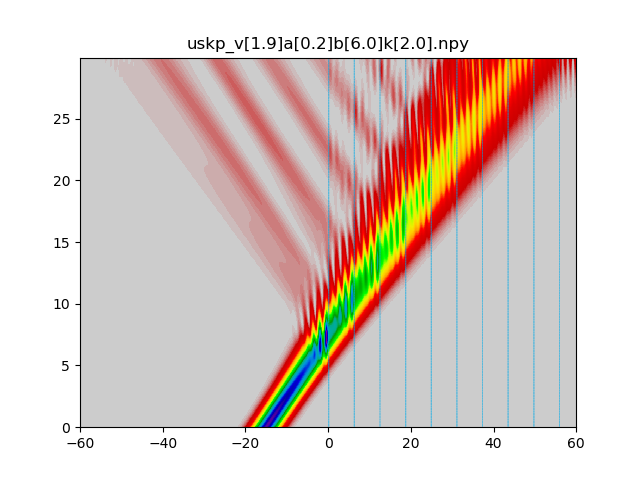
\includegraphics[width=0.9\hsize]{tajuhan1.png}
            \caption{高次反射波の例:壁が薄めのもの$V_0$=1.0, a=2.7, b=5.8}
            \label{thin}
        \end{minipage}
        \begin{minipage}{0.5\hsize}
            \centering
            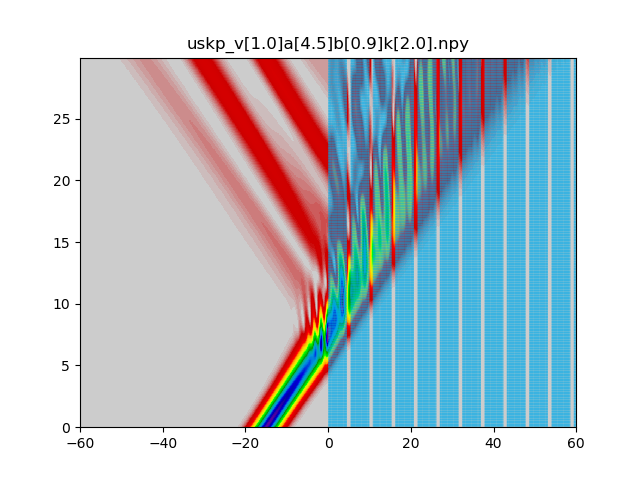
\includegraphics[width=0.9\hsize]{tajuhan2.png}
            \caption{高次反射波の例:壁が厚めのもの。停滞状態の影響がみられる$V_0$=1.0, a=4.5, b=0.9}
            \label{thick}
        \end{minipage}\\
        \begin{minipage}{0.5\hsize}
            \centering
            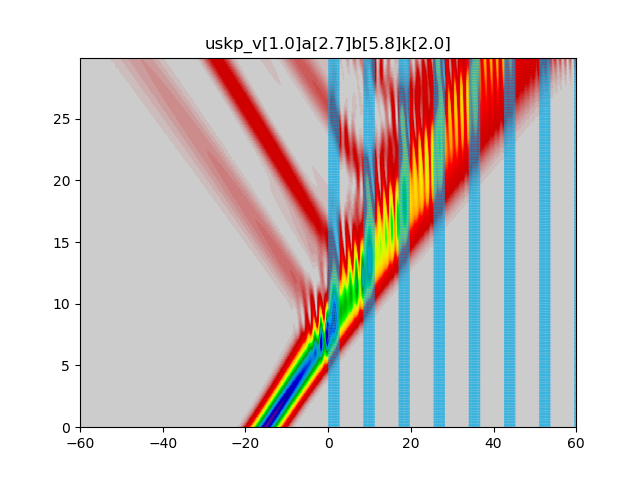
\includegraphics[width=0.9\hsize]{tajuhan3.png}
            \caption{高次反射波の例:2次の反射波が卓越している$V_0$=1.9, a=0.2, b=6.0}
        \end{minipage}
        \begin{minipage}{0.5\hsize}
            \centering
            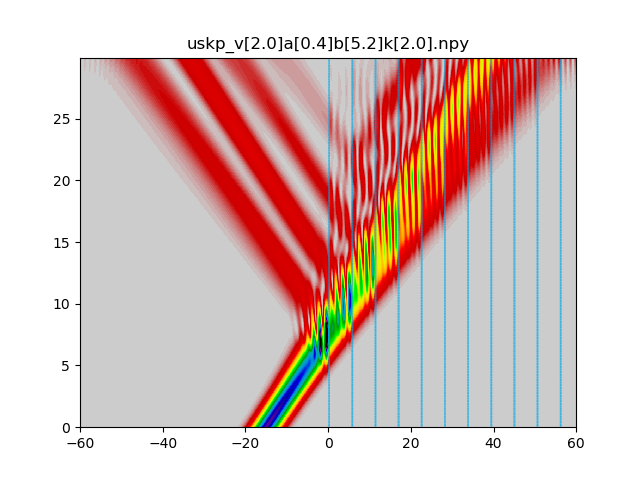
\includegraphics[width=0.9\hsize]{tajuhan4.png}
            \caption{高次反射波の例:2次進行波も同時に見られる珍しい例$V_0$=2.0, a=0.4, b=5.2}
        \end{minipage}
    \end{figure}
    \par ポテンシャルが$2.0$よりも低く, 壁が井戸に比べて薄い場合によくみられる。ポテンシャル表層だけでなく2層目や3層目でも反射波束が現れる。ほとんどが2回以上反射しない。
    \par 繰り返しをさけるため, n個目の反射波のことをn次反射波と呼ぶことにする。同様にn個目の進行波のことをn次進行波と呼ぶことにする。
    \par 高次反射波が表れる場合では1次反射波よりも2次反射波のほうが卓越している場合がみられる。\fref{thin}以外の例ではポテンシャル1層目内部で反射した2次反射波が最も卓越している。
    \par これは1次反射波と2次反射波の反射プロセスが違うためだと考えられる。まず, すべての例で1次反射波は真空-壁の境界付近で反射が起こっている。一方, \fref{thick}ではポテンシャル1層目で停滞する波が壁-井戸の境界で反射し, 再び真空へ侵入したものが2次反射波となる様子が観察できる。
    \par 二次反射波のほうが卓越しているパターンは壁が厚いものによくみられる。逆に壁が薄い\fref{thin}では1次反射波と2次反射波との間に大きな違いは見られない。
    \end{subsection}

    \begin{subsection}{高次進行波}
        \begin{figure}[h]
            \begin{minipage}{0.5\hsize}
                \centering
                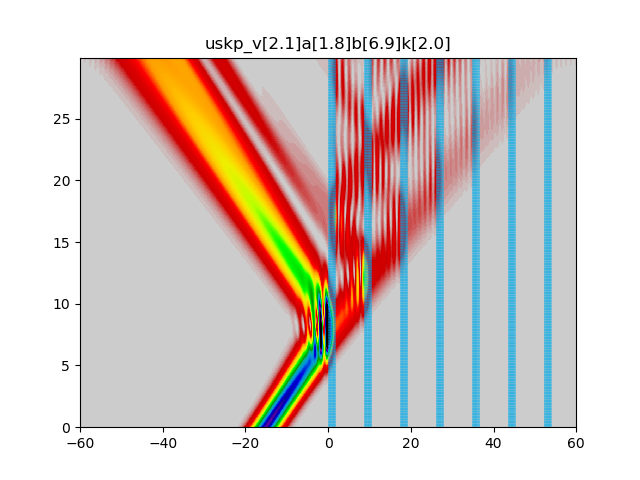
\includegraphics[width=0.9\hsize]{tajushin1.png}
                \caption{高次進行波の例:典型的なもの$V_0$=2.1, a=1.8, b=6.9}
                \label{temporal}
            \end{minipage}
            \begin{minipage}{0.5\hsize}
                \centering
                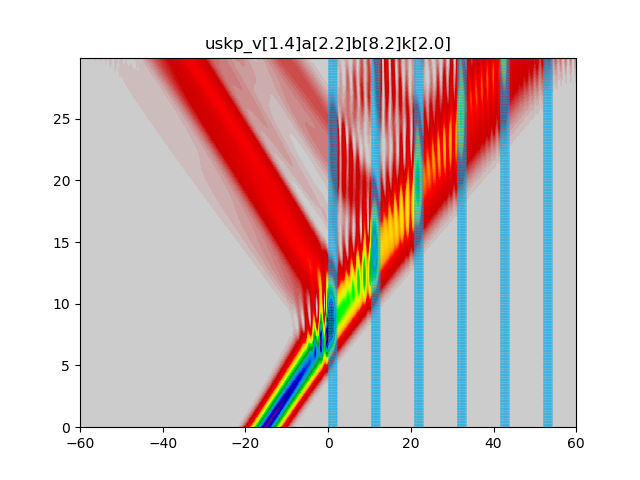
\includegraphics[width=0.9\hsize]{tajushin2.png}
                \caption{高次進行波の例:ひし形の模様がかなり大きく見える$V_0$=1.4, a=2.2, b=8.2}
                \label{thick_wide}
            \end{minipage}\\
            \begin{minipage}{0.5\hsize}
                \centering
                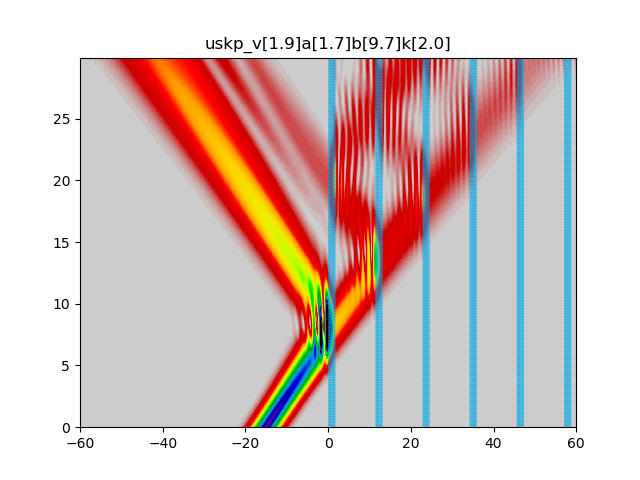
\includegraphics[width=0.9\hsize]{tajushin3.png}
                \caption{高次進行波の例:2次進行波が次第に卓越する様子が見られる$V_0$=1.9, a=1.7, b=9.7}
                \label{wide}
            \end{minipage}
            \begin{minipage}{0.5\hsize}
                \centering
                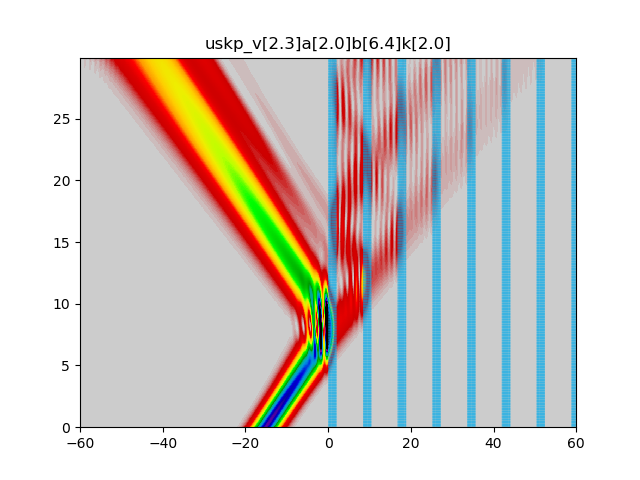
\includegraphics[width=0.9\hsize]{tajushin4.png}
                \caption{高次進行波の例:3次進行波も見られる珍しい例$V_0$=2.3, a=2.0, b=6.4}
                \label{narrow}
            \end{minipage}
        \end{figure}
    \par $V_0$=2前後, 壁の厚さが2程度, 井戸の幅が壁の倍以上のときにみられる。二層目以降の壁の左側で反射した波束がひとつ前の層の右側でもう一度反射して, はじめと同じ進行方向へ伝搬する。
    \par \fref{temporal}が最も分かりやすいが, 1次進行波は時間とともに減衰し, 2次進行波やそれ以降の波束が卓越していく。1次進行波が減衰する理由は, 全ての壁を透過する波が時間とともに減少する一方で, 新しく1次進行波に加わる波束が存在しないことがあげられる。一方で, 2次進行波は1次進行波から2回反射してきた波束が時間とともに加わってくる影響と, 2次進行波自身が壁で反射し減少する影響とが合わさるため, 単調に減衰するとはいえない。\fref{temporal}では20単位時間以降で2次進行波が卓越している。
    \par 進行波同士の時間的間隔は井戸の幅に影響を受ける。井戸の幅が広いと, 反射から反射までの時間的間隔が大きくなるため, 進行波同士の間隔も大きくなる。しかし, 波束がポテンシャル内で停滞する影響で, 反射そのものにかかる時間が存在する\cite{Goto}ため, 一概に井戸の幅だけに時間的間隔が依存しているとは言い切れない。実際に\fref{thick_wide}と\fref{wide}を比較すると\fref{wide}のほうが井戸が広い。しかし, \fref{wide}が3次反射波まで観察できる一方, \fref{thick_wide}では2次進行波までしか観察できない。これは単位時間当たりの反射回数が\fref{wide}のほうが多いことを意味している。ポテンシャルが厚くなると波束がポテンシャルに滞在する時間が伸びることの影響が表れていると考えられる。
    \end{subsection}

    \begin{subsection}{分裂状態}
        \begin{figure}[h]
            \begin{minipage}{0.5\hsize}
                \centering
                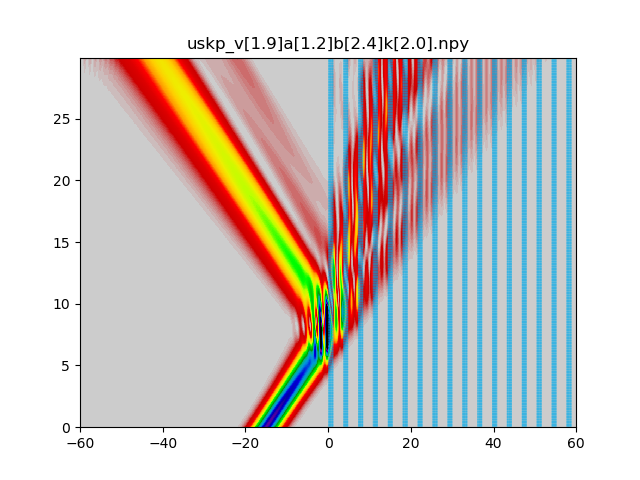
\includegraphics[width=0.9\hsize]{bunretsu1.png}
                \caption{分裂状態の例:分裂がいくつも起こっている$V_0$=1.9, a=1.2, b=2.4}
                \label{split_multi}
            \end{minipage}
            \begin{minipage}{0.5\hsize}
                \centering
                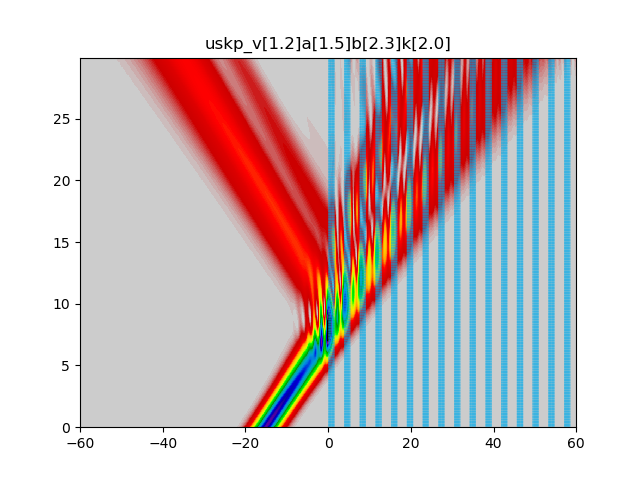
\includegraphics[width=0.9\hsize]{bunretsu2.png}
                \caption{分裂状態の例:壁が厚いもの$V_0$=1.2, a=1.5, b=2.3}
            \end{minipage}\\
            \begin{minipage}{0.5\hsize}
                \centering
                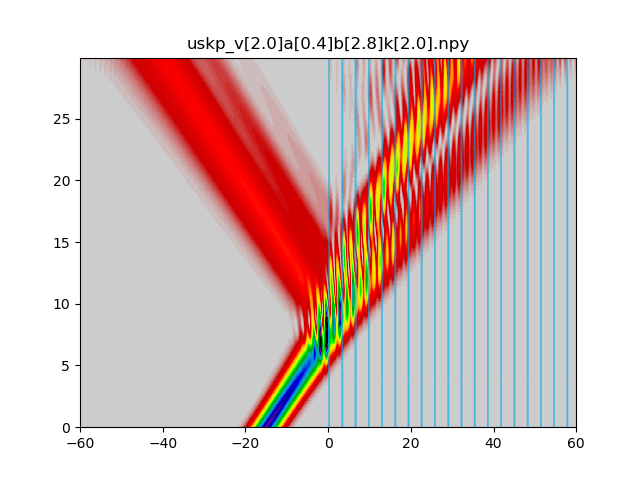
\includegraphics[width=0.9\hsize]{bunretsu3.png}
                \caption{分裂状態の例:2次反射波が卓越している$v_0$=2.0, a=0.4, b=2.8}
                \label{split_1}
            \end{minipage}
            \begin{minipage}{0.5\hsize}
                \centering
                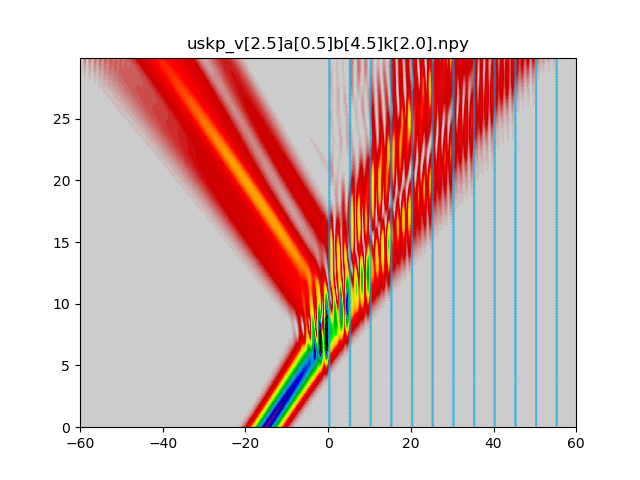
\includegraphics[width=0.9\hsize]{bunretsu4.png}
                \caption{分裂状態の例:2つの進行波が最も綺麗に分かれているもの$V_0$=2.5 , a=0.5, b=4.5}
            \end{minipage}
        \end{figure}
    \par ポテンシャルが2前後でよくみられる。ポテンシャルが高すぎるとみられなくなる。壁と井戸の関係に簡単な関係は見出されないが, 壁と井戸が同程度の場合に多く見られる。また, 壁が厚いと停滞の影響を受けて波束が分かれて見えないことが多い。
    \par ポテンシャルの内部に侵入した波束が二つ以上に分裂する。同時刻で切り取ると, 2つ以上の波束が固まって伝搬しているように見える。
    \par \fref{split_1}が最も分かりやすいが, 入射波と反射波が重なり合っているため, どの時刻で反射が起こるのかといった判別はできない。しかし, 全体として複数の進行波が伝搬しているように見える。
    \par 井戸の幅が大きくなると進行波同士の時間的間隔が大きくなるが, 2次進行波に含まれる波が少なくなる。逆に井戸の間隔が狭いと, 1次進行波がすぐに減衰する。そのため, 2次進行波と1次進行波が綺麗に分かれるには, 井戸が適度に広く, 1次進行波と2次進行波がどちらも減衰しないようなバランスが必要になる。
    \par また, \fref{split_multi}のように2次以上の高次の進行波が発生することも珍しくない。進行波は次第に減衰し, さらに高次の進行波が支配的になる。この様子は高次進行波の章で記述した内容と一致している。入射, 反射が絡みあった状態ながら, 全体として同様の傾向が見えることは非常に興味深い。
    \par さらに, 物質波波束において類似の現象が見られる\cite{Anker}が, これは物質波波束の非線形効果の影響と言われている。非線形効果を付加していない本研究での計算でも類似の現象が見られることも非常に興味深い。
    \end{subsection}

    \begin{subsection}{屈折状態}
        \begin{figure}[h]
            \begin{minipage}{0.5\hsize}
                \centering
                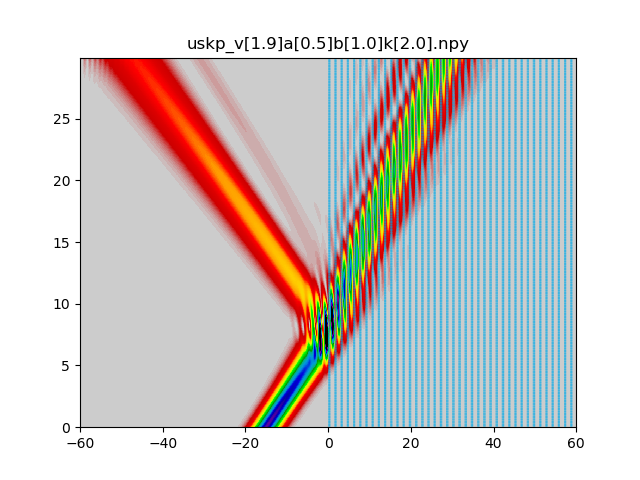
\includegraphics[width=0.9\hsize]{kussetsu1.png}
                \caption{屈折状態の例:周期が1.5のもの$v_0$=1.9, a=0.5, b=1.0}
            \end{minipage}
            \begin{minipage}{0.5\hsize}
                \centering
                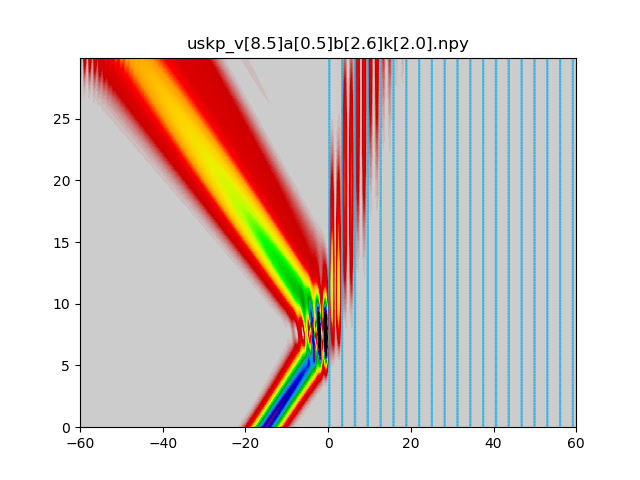
\includegraphics[width=0.9\hsize]{kussetsu2.png}
                \caption{屈折状態の例:周期が3.1のもの$v_0$=8.5, a=0.5, b=2.6}
            \end{minipage}\\
            \begin{minipage}{0.5\hsize}
                \centering
                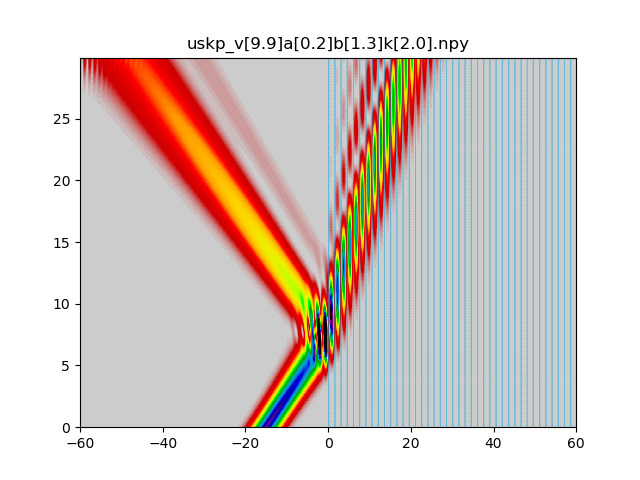
\includegraphics[width=0.9\hsize]{kussetsu3.png}
                \caption{屈折状態の例:ポテンシャルが高いもの$v_0$=9.9, a=0.2, b=1.3}
            \end{minipage}
            \begin{minipage}{0.5\hsize}
                \centering
                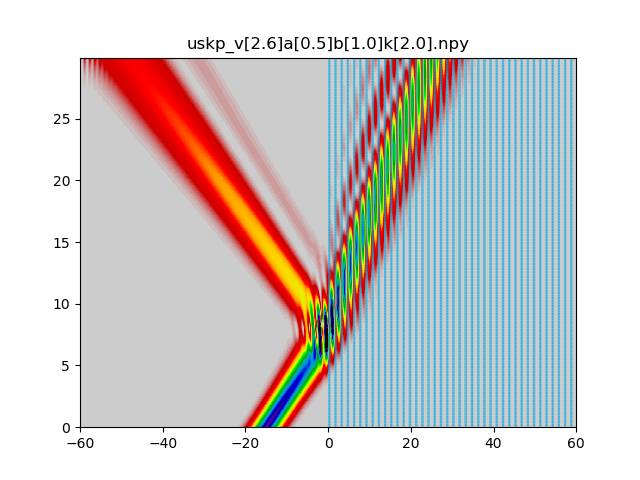
\includegraphics[width=0.9\hsize]{kussetsu4.png}
                \caption{屈折状態の例:進行波が最も一体として伝搬しているもの$v_0$=1.9, a=0.5, b=1.0}
            \end{minipage}
        \end{figure}
    \par ポテンシャルの周期が$1.5$, $3.1$などの場合にみられる。ポテンシャルの高さには関係せず, v=1.9からv=9.9の場合にまでみられた。波束がほぼ完全に一体となってポテンシャル中に入射している。特に$V_0$が5を超えるような設定では, ほとんどの場合で全反射が起こるが, 屈折状態だけは例外的に反射率が低い。
    \par ポテンシャルに入射した波束の傾きが, 真空中に比べて大きくなっていることから, 同じ位置に長時間滞在し続け, ゆっくり伝搬していく様子を見ることができる。
    \par 屈折状態が見られた周期はおおよそ$\pi$, $\pi/2$であり, de Broglie波長の平均に一致する。よって, この現象は何らかの形でポテンシャルと波束との共鳴的な現象が起こっていると考えられる。並進対称性がないにも関わらずBlochの定理のように逆格子定数のようなものが関わってくるならば, 非常に興味深い現象と言える。
    \end{subsection}

    \begin{subsection}{トラップ状態}
        \begin{figure}[h]
            \begin{minipage}{0.5\hsize}
                \centering
                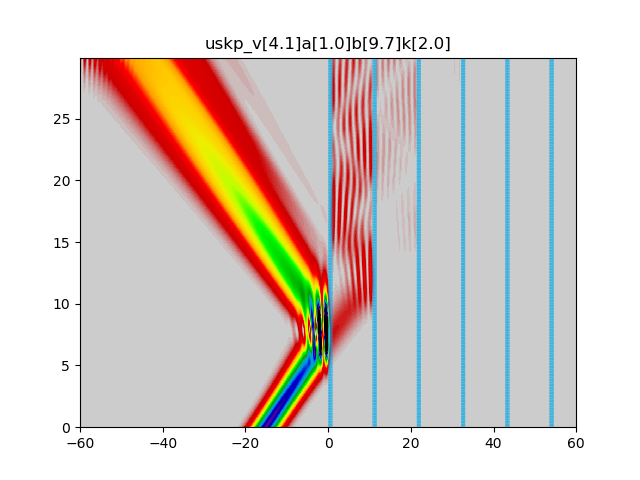
\includegraphics[width=0.9\hsize]{trap1.png}
                \caption{トラップ状態の例:1層目と2層目の間で反射し続けている$V_0$=4.1, a=1.0, b=9.7}
                \label{trap_tempo}
            \end{minipage}
            \begin{minipage}{0.5\hsize}
                \centering
                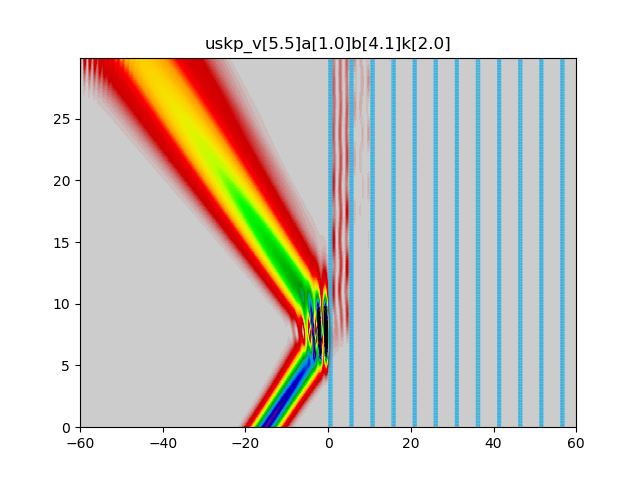
\includegraphics[width=0.9\hsize]{trap4.png}
                \caption{トラップ状態の例:井戸内で3つの腹が確認できる$V_0$=5.5, a=1.0, b=4.1}
                \label{trap3}
            \end{minipage}\\
            \begin{minipage}{0.5\hsize}
                \centering
                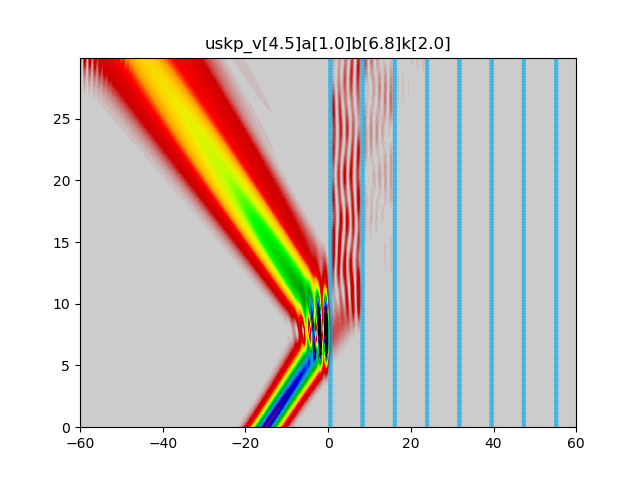
\includegraphics[width=0.9\hsize]{trap2.png}
                \caption{トラップ状態の例:井戸内で4つの腹が確認できる$V_0$=4.5, a=1.0, b=6.8}
                \label{trap4}
            \end{minipage}
            \begin{minipage}{0.5\hsize}
                \centering
                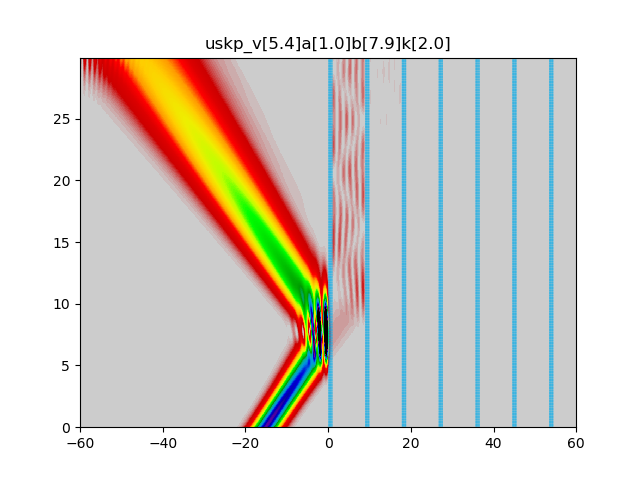
\includegraphics[width=0.9\hsize]{trap3.png}
                \caption{トラップ状態の例:井戸内で5つの腹が確認できる$V_0$=5.4, a=1.0, b=7.9}
                \label{trap5}
            \end{minipage}
        \end{figure}
    \par ポテンシャルが2よりも高く, 井戸と比較して壁が薄い場合にみられる。1層と2層の間に波束が入り, 出られなくなる。
    \par 3程度のポテンシャルの設定でトラップ状態のようなものが見られないわけではないが, ポテンシャルが5を超えるような高い設定の場合に$x-t$パターン上で縦縞模様が現れるような典型的なトラップ状態が見られる。5程度のポテンシャルの設定では, 壁が薄い場合にトラップ状態や分裂状態が見られ, 壁が厚くなるごとに全反射へと近づいていく。ポテンシャルが8程度になると全反射と屈折状態が支配的になり, トラップ状態のようなものは稀にしか見られない。
    \par また, \fref{trap_tempo}が分かりやすいが, トラップ状態といっても1層と2層の間に完全にとどまり続けることはなく, 次第に2層目と3層目の間に伝搬していく。
    \par \fref{trap3}では赤い領域が縦縞の様に3つ周期的に並んでおり, 共鳴のような構造が見られる。共鳴にならって確率密度が高くなっているところを腹と呼ぶことにする。\fref{trap3}, \fref{trap4}, \fref{trap5}と井戸の領域が広がるごとに, ひとつの井戸内に含まれる腹の数は増加しており, 「共鳴の波長」が井戸の幅によらないことが見受けられる。ガウス型波束の透過波が, あたかも切り取られた平面波のように振舞っているようにみえる様子は非常に興味深い。
    \par しかし, $x-t$パターンでは確率密度しか見取ることができないため, 位相の情報を得ることができない。確率密度が周期的に波打っていることは, トラップ状態の波動関数が平面波と類似していることを直接示すものではない。
    \end{subsection}

    \newpage

    \begin{subsection}{反射率と壁の厚さの関係}
        \par t=30の時点で真空領域に滞在している確率を波束の反射率として様々なパターンの反射率を計算した。結果を以下に示す。
        \begin{figure}[h]
            \centering
            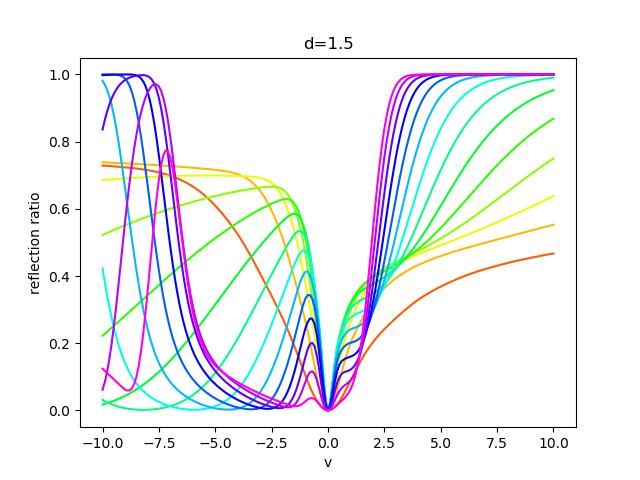
\includegraphics[width=10cm]{hansha.png}
            \caption{周期1.5のポテンシャルの反射率}
            \label{hansha}
        \end{figure}
        \par 曲線の色は1周期における壁の割合を示している。赤から紫にわたって虹のスペクトルと同じ順番で壁の割合が高くなっている。
        \par 注目すべきはV=1.9周辺で, 反射率が最も高いものが緑色(壁の割合が50\%程度)であり, 赤色(壁の割合が3\%)や紫(壁の割合が97\%)はそれよりも低い。古典的な発想ではポテンシャルが高いほど反射率も高くなりそうだが, シミュレーション結果はそのようにはならない。
        \par 比較のために箱型ポテンシャルの定常状態について, 壁の幅を対応させた形で同様のグラフを作成したところ, \fref{hako}を得た。
        \newpage
        \begin{figure}[h]
            \centering
            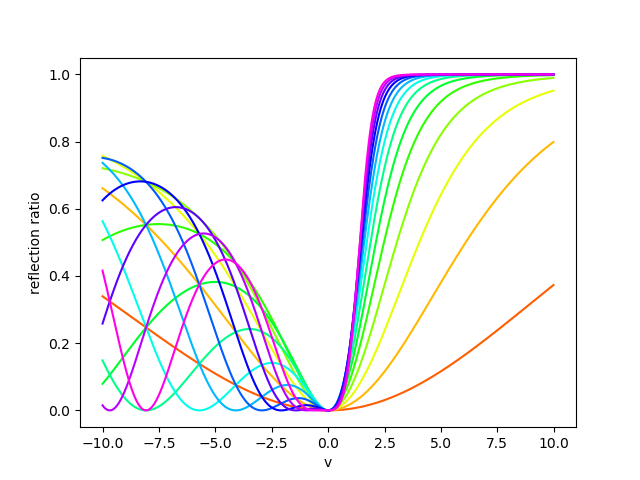
\includegraphics[width=10cm]{hako.png}
            \caption{箱型ポテンシャルの定常状態における反射率}
            \label{hako}
        \end{figure}
        \par \fref{hako}では\fref{hansha}のような逆転現象は見られない。これは反射率の定義の違いによるものと考えられる。\fref{hansha}では30単位時間後という有限の時間が経過した時点の真空領域に粒子が存在する確率を反射率の定義にしているが, \fref{hako}では定常状態という, 無限の時間が経過した状態における真空領域での進行波と後退波の振幅の比によって定義している。
        \par 有限の時間では, セクション\ref{teitais}で述べたように壁内部に波が停滞し, 長い時間スケールに渡ってゆっくりと波が放出される現象の影響を受ける。\fref{hansha}において, 壁が非常に厚くなった場合に反射率が低くなる現象が見られる理由は, 停滞状態が関係していると考えられる。停滞状態のパターンのようにポテンシャル内から出てこなくなっている粒子が一定数存在すると, 有限時間での反射率は低く見積もられる。
    \end{subsection}
\end{section}

\newpage

\begin{section}{結論}
    \par 波束の時間発展に関して, 最適化されたコードを実行するためのフレームワークQantumSketchBookの作成を行った。これによって, Schrödinger方程式の初期値問題の求積と可視化を7行で記述できるようなフレームワークを作成することが出来た。
    \par QSBの妥当性を検証するためにZhangの計算を再計算した。その結果, 二つの計算方法でほぼ同様の結果を得られたことが確認できたため, QSBの計算について, ある程度の妥当性を保証することができた。
    \par QSBを用いてKronig-Pennyポテンシャルに入射するGauss型波束の時間発展を5000ケース以上シミュレーションした。このような大量のケースを計算することが可能となったのは, フレームワークによって効率化されたプログラムを簡単に再利用することが可能になったからである。フレームワークを活用することの恩恵を十分に受けることができたといえる。
    \par $x-t$パターンを作成したところ, 特徴的な7パターンを抽出することが出来た。
    \par 停滞状態では直感に反してポテンシャル領域に長時間滞在する粒子が存在することを見取ることができた。これは時間発展する粒子の興味深い性質の一つである。
    \par また, 2個以上の波束が真空領域へ反射する高次反射波の現象を見取ることができた。特に1次反射波よりも2次反射波が卓越することと停滞状態との関係を見いだすことが出来たことは, 今回見取ることができた量子波束の興味深い性質の一つといえる。
    \par 更に, 高次進行波の時間的間隔が単純な井戸の距離だけでは表されず, 反射そのものにかかる時間も影響することを匂わせる現象が見られたことも興味深い結果と言える。
    \par 分裂状態では入射波と反射波の影響が絡み合っている状況でも波束が全体として進行波のように伝搬していく様子を確認できた。また, 非線形項の影響が入っていないにも関わらず, 波束が2つ以上に分裂していく現象は直感的に予想することが難しい現象の一つと言える。
    \par 屈折状態では, 一定の周期を持つポテンシャルで, ポテンシャルの高さに関係なく類似の現象が見られたことは, 何らかのポテンシャル構造に関する普遍性を示すものとして興味深い。また, 高いポテンシャルの設定でも透過率の高い状況を選択的に作り出すことができる可能性を与えるこの結果は, 実用的な応用を微かに期待させる。
    \par トラップ状態では様々な波数の波が重なり合っているはずの波束において, ひとつの周波数を持っているような振る舞いが見られた。波束の振る舞いについてのひとつの知見を得ることが出来たと考えられる。
    \par 最後に, 壁の厚さと反射率の関係では, 壁が厚くなるほど反射率が下がる場合があるという, 直感とは反する結果が得られた。有限の時間内に起こる反射と定常状態における反射の違いが問題になる場合の例を一つ提供することができたと考えられる。
    \par 本研究では, フレームワークの有効性を示したことと波束の時間発展に関する興味深い現象の知見を得たことという, 二つの成果が得られたと考えられる。
\end{section}

\appendix

\begin{section}{Blochの定理の簡単な証明\label{AppB}}
    \par ハミルトニアンHに以下の条件を課す。$T_d$は移動距離$d$の並進演算子。
    \begin{align}
     [T_d, H]=0\nonumber\\
    \end{align}
    \par これは並進対称性を表している。これにより, 固有状態$\phi$は$d$の整数倍の周期を持ち, $H$と$T_d$の同時固有状態になる。並進演算子の固有状態は1の整数乗根になる。
    \begin{align}
     T_d\phi=A\phi\nonumber\\
        (T_d)^n\phi=A^n\phi=\phi\nonumber\\
        A=\mathrm{e}^{i2\pi/n}=\mathrm{e}^{iKd}\nonumber\\
        K=\frac{2\pi}{n d}
    \end{align}
    \par $\phi$の周期を$nd$とした。ここで以下の関数$u$を考える。
    \begin{align}
     u(x) &= \mathrm{e}^{iKx}\phi(x)\label{ux}\nonumber\\
    \end{align}
    \begin{align}
     T_d u(x) &= \mathrm{e}^{iK(x-d)}\mathrm{e}^{iKd}\phi(x)\nonumber\\
        T_d u(x) &= \mathrm{e}^{iKx}\phi(x)=u(x)
    \end{align}
    \par よって$u(x)$は周期$d$を持つ周期関数だということが分かる。
    \par $u(x)$の定義を変形すればBlochの定理を証明したことになる。
    \begin{align}
     \phi(x) = \mathrm{e}^{-iKx}u(x)\nonumber\\
    \end{align}
    \par $K$を三次元に拡張したものは逆格子ベクトルと呼ばれる。
\end{section}

\begin{section}{Kronig-Pennyモデルのエネルギーバンド構造の簡単な計算方法\label{AppK}}
    \par 井戸と壁のSchrödinger方程式は単純な単振動になるため, エネルギーを$\varepsilon$としたとき以下のような解になる。
    \begin{align}
     \phi_{well}(x)=W^+\mathrm{e}^{+ikx}+W^-\mathrm{e}^{-ikx}\nonumber\\
        \phi_{barrier}(x)=B^+\mathrm{e}^{+iqx}+B^-\mathrm{e}^{-iqx}\nonumber\\
        k=\sqrt{2m\varepsilon}\nonumber\\
        q=\sqrt{2m(\varepsilon - V_0)}
    \end{align}
    \par $W^+$, $W^-$, $B^+$, $B^-$は振幅を表す定数。
    \par $\phi(x)$に一回微分までの連続性を課すと, 井戸と壁の境界で以下の条件が必要となる。
    \begin{align}
     \begin{pmatrix} 1 & 1 \\ 1 & -1 \end{pmatrix}\begin{pmatrix} W^{ + } \\ W^{ - } \end{pmatrix}=\begin{pmatrix} 1 & 1 \\ \rho & -\rho \end{pmatrix}\begin{pmatrix} B^{ + } \\ B^{ - } \end{pmatrix}\nonumber\\
    \end{align}
    \begin{align}
     \begin{pmatrix} \mathrm{e}^{ika} & \mathrm{e}^{-ika} \\ \mathrm{e}^{ika} & -\mathrm{e}^{-ika} \end{pmatrix}\begin{pmatrix} W^{+} \\ W^{-} \end{pmatrix}=\begin{pmatrix} \mathrm{e}^{iqa} & \mathrm{e}^{-iqa} \\ \rho\mathrm{e}^{iqa} & -\rho \mathrm{e}^{-iqa} \end{pmatrix}\begin{pmatrix} B^{+} \\ B^{-} \end{pmatrix}\nonumber\\
    \end{align}
    \par ここで$\rho=q/k$。
    \par Blochの定理を上式の左辺に使うと以下の置き換えをすることができる。
    \begin{align}
        \mathrm{e}^{ika}\rightarrow\mathrm{e}^{ikb}\mathrm{e}^{-iKd}\\
        \mathrm{e}^{-ika}\rightarrow\mathrm{e}^{-ikb}\mathrm{e}^{-iKd}
    \end{align}
    \end{section}
    簡略のために以下の置換えをする。
    \begin{align}
     H&=\begin{pmatrix} 1 & 1 \\ 1 & -1 \end{pmatrix}\nonumber\\
        \alpha &=\begin{pmatrix} 1 & 0 \\ 0 & \rho  \end{pmatrix}\nonumber\\
        K_x&=\begin{pmatrix} \mathrm{e}^{ikx} & 0 \\ 0 &  \mathrm{e}^{-ikx} \end{pmatrix}\nonumber\\
        Q_x&=\begin{pmatrix} \mathrm{e}^{iqx} & 0 \\ 0 &  \mathrm{e}^{-iqx} \end{pmatrix}\nonumber\\
        \mathbf{W}& = \begin{pmatrix} W^{+} \\ W^{-} \end{pmatrix}\nonumber\\
        \mathbf{B}& = \begin{pmatrix} B^{+} \\ B^{-} \end{pmatrix}
    \end{align}
    ちなみに, HはHadamard行列として知られている。
    置き換えをすると以下のような式が得られる。
    \begin{align}
     H \mathbf{W} - H \alpha \mathbf{B} = 0\nonumber\\
        \mathrm{e}^{-iKd} K_b H \mathbf{W} - Q_a H \alpha \mathbf{B} = 0
    \end{align}
    整理すると以下のような方程式が得られる。
    \begin{align}
     \begin{pmatrix} E & \alpha  \\ E & { e }^{ iKd }H^{ -1 }K_{ b }^{ -1 } Q_{ a }H\alpha  \end{pmatrix}\begin{pmatrix} \mathbf{ W } \\ \mathbf{ B } \end{pmatrix}=0\nonumber\\
    \end{align}
    ここで$E$は2次の単位行列。
    トリビアルでない解は行列部分が0となるときに現れる。4行4列の行列式を求める手続きは煩雑だが, 余因子展開を繰り返せば必ず展開できる。幸い, 今回は単位行列が現れることを利用すれば, 実質的に現れる項は4項だけとなる。

\begin{section}{定常状態の計算\label{AppT}}
    \par 数値計算で用いたポテンシャルにおける定常解は転送行列によって扱うことができる。
    \begin{align}
     V(x)=\begin{cases}0&(x<0)\\V_{KP}(x)&(x>0)\end{cases}\nonumber\\
    \end{align}
    \par Schrödinger方程式の解はKronig-Pennyモデルの計算と同じ形になる。連続の条件を課すと, 以下の境界条件が成立する。
    \begin{align}
     K_{dn} H \mathbf{W_n} = Q_{dn} H \alpha \mathbf{B_n}\nonumber\\
        K_{a} K_{dn} H \mathbf{W}_{n+1} = Q_a Q_{dn} H \alpha \mathbf{B}_n
    \end{align}
    \par 前章で用いた置き換えを使った。$W_n$, $b_n$は0から数えて原点からn周期目の井戸, 壁における振幅を表している。
    \par 上式から井戸の振幅についての漸化式を作ると以下のようになる。
    \begin{align}
     \mathbf{W}_{n+1}= H^{-1} K_{dn}^{-1} K_a^{-1} Q_a K_{dn} H \mathbf{W}_n\nonumber\\
    \end{align}
    \par ちなみに, 一般項は以下のようになる。
    \begin{align}
     \mathbf{W}_n = H^{-1} \left( K_b Q_a \right)^n H \mathbf{W}_0\nonumber\\
    \end{align}
    \par 初項$W_0$を漸化式の係数部分$A = H^{-1} K_{dn}^{-1} K_a^{-1} Q_a K_{dn} H$の固有ベクトル$A_1$, $A_2$で展開する。ここで, 固有値$a_1$, $a_2$ には$|a_1|<|a_2|$の関係があることにする。
    \begin{align}
     \mathbf{W}_n = c_1 A_1 + c_2 A_2\nonumber\\
      W_0 = A^{-n} W_n = c_1 a_1^{-n} A_1 + c_2 a_2^{-n} A_2
    \end{align}
    \par ここで, $n \rightarrow \infty$の場合を考えると, $|a_1|^{-n}>>a_2^{-n}$となり, $W_0$の主成分は$A_1$となる。
    \par $A_1$における進行波と後退波の比をとれば, 反射率を得ることができる。
\end{section}

\begin{section}{QSBのソースコード}
    QSBソースコードはいくつかのテストコードとともにインターネット上でもMITライセンスで公開されている\cite{QSB}。

    \lstinputlisting[caption=\_\_init\_\_.py]{__init__.py}
    \lstinputlisting[caption=mesh.py]{mesh.py}
    \lstinputlisting[caption=context.py]{context.py}
    \lstinputlisting[caption=quantized.py]{quantized.py}
    \lstinputlisting[caption=field.py]{field.py}
    \lstinputlisting[caption=potential.py]{potential.py}
    \lstinputlisting[caption=stste.py]{state.py}
    \lstinputlisting[caption=laplasian.py]{laplasian.py}
    \lstinputlisting[caption=hamiltonian.py]{hamiltonian.py}
    \lstinputlisting[caption=schroedinger.py]{schroedinger.py}
\end{section}

\begin{thebibliography}{30}
    \bibitem{Kittel}Kittel, C. (1976). Introduction to solid state physics. New York: Wiley, 1976, 5th ed., 1.
    \bibitem{Bloch}Bloch, F. (1929). Über die quantenmechanik der elektronen in kristallgittern. Zeitschrift für physik, 52(7-8), 555-600.
    \bibitem{KP}Kronig, R. D. L., \& Penney, W. G. (1931, February). Quantum mechanics of electrons in crystal lattices. In Proceedings of the Royal Society of London A: Mathematical, Physical and Engineering Sciences (Vol. 130, No. 814, pp. 499-513). The Royal Society.
    \bibitem{Nagaoka}長岡洋介. (1985). アンダーソン局在. 日本物理学会誌, 40(7), 489-498.
    \bibitem{Esaki}Esaki, L., \& Tsu, R. (1970). Superlattice and negative differential conductivity in semiconductors. I B M J RES DEVELOP, 14(1), 61-65.
    \bibitem{Szmulowicz}Szmulowicz, F. (1997). New eigenvalue equation for the Kronig–Penney problem. American Journal of Physics, 65(10), 1009-1014.
    \bibitem{nobelAnderson}Nobelprize.org, (2018/1/20閲覧),The Nobel Prize in Physics 1977, https://www.nobelprize.org/nobel\_prizes/physics/laureates/1977/
    \bibitem{nobelEsaki}Nobelprize.org, (2018/1/20閲覧),The Nobel Prize in Physics 1973, https://www.nobelprize.org/nobel\_prizes/physics/laureates/1973/
    \bibitem{Anker}Anker, T., Albiez, M., Eiermann, B., Taglieber, M., \& Oberthaler, M. K. (2004). Linear and nonlinear dynamics of matter wave packets in periodic potentials. Optics express, 12(1), 11-18.
    \bibitem{Katori}Yamanaka, K., Ohmae, N., Ushijima, I., Takamoto, M., \& Katori, H. (2015). Frequency Ratio of Hg 199 and Sr 87 Optical Lattice Clocks beyond the SI Limit. Physical review letters, 114(23), 230801.
    \bibitem{Zhang}Zhang, Z., Tong, P., Gong, J., \& Li, B. (2012). Quantum hyperdiffusion in one-dimensional tight-binding lattices. Physical review letters, 108(7), 070603.
    \bibitem{Koide}小出昭一郎, (2008), 量子力学I改訂版, 裳華房, 基礎物理学選書, 5A, 50版 など
    \bibitem{Huf}Hufnagel, L., Ketzmerick, R., Kottos, T., \& Geisel, T. (2001). Superballistic spreading of wave packets. Physical Review E, 64(1), 012301.
    \bibitem{Moyer}Moyer, C. A. (2004). Numerov extension of transparent boundary conditions for the Schrödinger equation in one dimension. American Journal of Physics, 72(3), 351-358.
    \bibitem{Maeda}前田雅人(2014).量子波束の跳ね返りシミュレーション.卒業論文
    \bibitem{Hosaka}保坂あゆみ, (2011).2次元ポテンシャル障壁を透過する波束の運動と量子軌道.卒業論文
    \bibitem{Goto}後藤敬佑 (2015).確率力学に基づいた量子跳ね返り時間のシミュレーション.卒業論文
    \bibitem{Futohashi}太箸良介 (2015).相対論的粒子の量子跳ね返り時間.卒業論文
    \bibitem{QSB} https://github.com/tmaeda11235/schroedinger\_solver で開発版のソースコードを公開している
    \bibitem{Pavelich}Pavelich, R. L., \& Marsiglio, F. (2015). The Kronig-Penney model extended to arbitrary potentials via numerical matrix mechanics. American Journal of Physics, 83(9), 773-781.
    \bibitem{python}python.org, (2018/1/19閲覧) Python 3.6.3 ドキュメント, https://docs.python.jp/3/index.html
    \bibitem{scipy}scipy.org, (2018/1/19閲覧), Scipy Lecture Notes, http://www.scipy-lectures.org/
    \bibitem{pep8}pyton.org, (2018/1/19閲覧), PEP 8 -- Style Guide for Python Code, https://www.python.org/dev/peps/pep-0008/
    \bibitem{pep484}pyton.org, (2018/1/19閲覧), PEP 484 -- Type Hints, https://www.python.org/dev/peps/pep-0484/
    \bibitem{pep20}pyton.org, (2018/1/19閲覧), PEP 20 -- The Zen of Python, https://www.python.org/dev/peps/pep-0020/
    \bibitem{Carnahan}Carnahan, B.\&Luther\&H.A., Wilkes, J.O., 藤田宏他訳(1982).計算機による数値計算法, 日本コンピュータ協会, コンピュータ・サイエンス研究書シリーズ / 日本コンピュータ協会編, 19
    \bibitem{Siegle}Siegle, P., Goychuk, I., \& Hänggi, P. (2010). Origin of hyperdiffusion in generalized brownian motion. Physical review letters, 105(10), 100602.
\end{thebibliography}

\end{document}
